% ====================================================================
% JMP_seminar_beamer_v19.tex -- seminar deck, V19 literature and presentation
% refinement.  V18, V17, V16 and r6 are kept intact.
%
% Economics-first main deck: scope is stated once, on the scope slide; the
% qualifications live in speaker notes and backup slides.  New: the
% inequality-of-opportunity positioning (two slides), building blocks, the
% identification strategy, and backups for the benchmark table, literature,
% observational equivalence, the attained-bundle numerical design, the prospect
% reference and parameter uncertainty.
%
% Numbers: every numeral is a macro from deck_numbers_v19.tex
% (`make_deck_numbers_r6.py --v19`).  The paper's numbers come from the V15
% registry; literature numbers come from literature_benchmarks_v19.json and are
% re-verified against the literature corpus at build time.  Figures: V15 image
% files, unchanged.  Checks: `verify_deck_r6.py --deck v19`.  Build: build_deck_v19.py.
% ====================================================================
\documentclass[10pt,aspectratio=169]{beamer}
% ====================================================================
% jmp_beamer_preamble.tex --- shared preamble for the JMP seminar deck.
%
% REUSED VERBATIM from the companion theory talk
%   beamer/reference/Theory_talk/slides/Presentation.tex
%     "Jobs and Well-Being Measurement" (Haydar and Maniquet)
% so that the two decks read as one visual family.  The elements carried
% over unchanged are marked [THEORY-TALK] below; everything else is an
% addition this deck needs and the theory talk does not.
%
% Consistency is the point: same class options, same theme, same accent
% colour, same frame numbering, same appendix handling, same visible-link
% convention, same note-page template, same two-agent sketch palette.
% ====================================================================

% ---- [THEORY-TALK] class, theme and the deep-red accent -------------
\usetheme{metropolis}
\definecolor{deepred}{RGB}{150,25,35}
\setbeamercolor{frametitle}{bg=deepred}
\setbeamertemplate{navigation symbols}{}
% metropolis-defined accents (safe: these beamercolors exist in metropolis)
\setbeamercolor{progress bar}{fg=deepred}
\setbeamercolor{title separator}{fg=deepred}
% frame number as current/total, in deep red
\metroset{numbering=fraction}
\setbeamercolor{footline}{fg=deepred}
% backup appendix: keep the main frame total at the running-order count
\usepackage{appendixnumberbeamer}
% VISIBLE link colours for rehearsal (internal hyperlinks in deep red)
\hypersetup{colorlinks=true,linkcolor=deepred,citecolor=deepred,urlcolor=deepred}

% ---- [THEORY-TALK] encoding, language, maths, tables, tikz ----------
\usepackage[utf8]{inputenc}
\usepackage[english]{babel}
\usepackage{amsmath}
\usepackage{amssymb}
\usepackage{amsfonts}
\usepackage{booktabs}
\usepackage[official]{eurosym}   % \euro --- this deck quotes euro magnitudes
\usepackage{tikz}
\usetikzlibrary{decorations.pathreplacing,arrows.meta,positioning,fit,backgrounds}

% ---- [THEORY-TALK] the two-agent sketch palette --------------------
% red = agent i / household A ; blue = agent h / household B
\definecolor{agenti}{RGB}{200,30,40}
\definecolor{agenth}{RGB}{20,80,200}

% ---- [THEORY-TALK] notes on a second screen (rehearsal view) -------
% The rehearsal build turns this on; the projection build leaves it off.
\usepackage{pgfpages}
% Long notes overflow the note column by default; render them smaller,
% ragged-right, with tight paragraph spacing so the full text stays
% legible and inside the frame on the second screen.
%
% This deck's notes are longer than the theory talk's -- several run past
% one note page at \scriptsize and produced overfull \vbox warnings.  The
% template below keeps the theory talk's look and adds two things it
% needs: \tiny with a tighter baseline, and an \allowbreak-friendly
% vertical box so a long note breaks across note pages instead of
% overflowing.  Hyphenation is relaxed so no line runs into the margin.
\setbeamertemplate{note page}{%
  \vspace{0.3em}\par
  {\tiny\setlength{\parskip}{0.45em}\setlength{\parindent}{0pt}%
   \setlength{\emergencystretch}{3em}%
   \linespread{1.05}\selectfont
   \raggedright\insertnote\par}%
}
% Notes are prose, not code: let TeX hyphenate freely rather than push a
% long word past the measure.
\hyphenpenalty=50
\tolerance=2000

\DeclareMathOperator*{\argmax}{arg\,max}

% ====================================================================
% ADDITIONS for this deck (not in the theory talk)
% ====================================================================

% ---- channel colours ------------------------------------------------
% One colour per decomposition channel, used consistently on every slide
% that names a channel.  Preferences take the theory talk's agent-red so
% the two decks agree on which side of the argument is which.
\definecolor{chpref}{RGB}{200,30,40}     % preferences   (= agenti)
\definecolor{chacc}{RGB}{20,80,200}      % job access    (= agenth)
\definecolor{chearn}{RGB}{200,120,20}    % earning opportunities
\definecolor{chneeds}{RGB}{40,120,70}    % endowments and needs
\definecolor{chenv}{RGB}{60,60,70}       % the whole environment

% ---- the paper's notation ------------------------------------------
% Audience-facing channel names are WORDS on the slides; these commands
% exist so the words are spelled the same way every time they appear.
\newcommand{\pref}{\textcolor{chpref}{preferences}}
\newcommand{\Pref}{\textcolor{chpref}{Preferences}}
\newcommand{\acc}{\textcolor{chacc}{job access}}
\newcommand{\Acc}{\textcolor{chacc}{Job access}}
\newcommand{\earn}{\textcolor{chearn}{earning opportunities}}
\newcommand{\Earn}{\textcolor{chearn}{Earning opportunities}}
\newcommand{\needs}{\textcolor{chneeds}{household endowments and needs}}
\newcommand{\Needs}{\textcolor{chneeds}{Household endowments and needs}}
\newcommand{\env}{\textcolor{chenv}{the environment}}
\newcommand{\Env}{\textcolor{chenv}{The environment}}

% Symbols.  The theory-paper symbols W, z, R, A, y appear ONLY where the
% companion paper is cited; the estimation notation is separate.
\newcommand{\Wmeasure}{W}                      % theory-paper measure
\newcommand{\Jset}{\mathcal{J}}                % theory-paper job space
\newcommand{\Wone}{W^{1}}                      % theory-paper W^1
\newcommand{\yref}{\mathbf{y}^{w}}             % theory-paper reference pay
\newcommand{\gopp}{g}                          % estimated offer density
\newcommand{\uutil}{u}                         % preference index
\newcommand{\Wmm}{\mathrm{W}}                  % money-metric welfare level

% ---- headline / caveat call-outs -----------------------------------
\newcommand{\headline}[1]{{\large\textcolor{deepred}{#1}}}
\newcommand{\caveat}[1]{{\footnotesize\textcolor{deepred}{#1}}}
% a number with its numerical-integration band
\newcommand{\wband}[2]{#1\,\ensuremath{\pm}\,#2}

% ---- the 25-minute variant ------------------------------------------
% Every frame carries \shortdeck (in the 25-minute running order) or
% \longdeck (45-minute only).  \DeckShort, set by the driver file, drops
% the \longdeck frames; the default keeps everything.
%
% The frozen plan's 25-minute running order is 16 slides, reached from the
% 23 by FIVE cuts and TWO merges:
%   CUT   -> backup : 9, 12, 17, 18, 22          (\longdeck)
%   MERGE           : 6+7 -> one slide, 10+11 -> one slide
% So three tags, not two.  A merged pair is written as two full frames for
% the 45-minute deck; in the short deck the SECOND of the pair drops and
% the first shows its merged content.  23 - 5 - 2 = 16.
%
% Usage:  \shortdeck{\begin{frame}...\end{frame}}     kept in both
%         \longdeck{\begin{frame}...\end{frame}}      45-minute only (cut)
%         \mergedaway{\begin{frame}...\end{frame}}    45-minute only (merged)
%         \ifDeckShort ... \else ... \fi              inline merged content
\newif\ifDeckShort\DeckShortfalse
\newcommand{\shortdeck}[1]{#1}                       % always kept
\newcommand{\longdeck}[1]{\ifDeckShort\else#1\fi}    % cut to backup at 25 min
\newcommand{\mergedaway}[1]{\ifDeckShort\else#1\fi}  % folded into the previous
% content shown only in the merged (25-minute) form of a slide
\newcommand{\mergedonly}[1]{\ifDeckShort#1\fi}

% ---- figure helper ---------------------------------------------------
% Every figure is a PDF from the frozen sprint set, included by name from
% beamer/figures/.  \deckfig{name}{width fraction} keeps the call sites
% uniform and makes a missing file fail loudly at compile time.
\graphicspath{{figures/}}
% Heights leave room for the frametitle, the one caption line every figure
% slide carries, and the metropolis footline -- a taller box overflows the
% frame and shows up as an overfull \vbox.
\newcommand{\deckfig}[2]{%
  \begin{center}\includegraphics[width=#2\textwidth,height=0.70\textheight,%
    keepaspectratio]{#1}\end{center}}
\newcommand{\deckfigtwo}[4]{%
  \begin{columns}[c,onlytextwidth]
  \column{0.49\textwidth}\includegraphics[width=\textwidth,height=0.60\textheight,%
    keepaspectratio]{#1}\\{\centering\scriptsize #2\par}
  \column{0.49\textwidth}\includegraphics[width=\textwidth,height=0.60\textheight,%
    keepaspectratio]{#3}\\{\centering\scriptsize #4\par}
  \end{columns}}

% ---- tables ---------------------------------------------------------
% Several slides carry a comparison table that is naturally wider than the
% text block.  \decktable shrinks one to the measure rather than letting it
% run into the margin (an overfull \hbox), and never enlarges a narrow one.
\newcommand{\decktable}[1]{%
  \begin{center}\resizebox{\textwidth}{!}{#1}\end{center}}

\endinput

\usepackage{array}
% deck_numbers_v19.tex -- GENERATED by make_deck_numbers_r6.py --v19.
% Do not edit by hand.  The paper's numbers: V15 registry entries, gallery fields
% or recorded ratios of them.  Literature numbers: literature_benchmarks_v19.json,
% re-verified against the literature corpus.

\newcommand{\VCollectionYear}{2016}
\newcommand{\VIncomeYear}{2015}
\newcommand{\VNSingles}{1,540}
\newcommand{\VNCouples}{2,223}
\newcommand{\VCEqGiniSingles}{0.2633}
\newcommand{\VAttEqGiniSingles}{0.2498}
\newcommand{\VCEqGiniCouples}{0.2268}
\newcommand{\VAttEqGiniCouples}{0.1974}
\newcommand{\VKFreeSingles}{41}
\newcommand{\VKFreeRumA}{10}
\newcommand{\VKFreeRumB}{16}
\newcommand{\VRumGap}{141.64}
\newcommand{\VMaeSingles}{0.0140}
\newcommand{\VMaeRumA}{0.0273}
\newcommand{\VMaeRumB}{0.0264}
\newcommand{\VMatchedAccessRatio}{14.5}
\newcommand{\VMatchedWageGap}{11.5}
\newcommand{\VMatchedEmpShareA}{0.75}
\newcommand{\VMatchedEmpShareB}{0.17}
\newcommand{\VEAOppMin}{7.9}
\newcommand{\VEAOppMax}{21.3}
\newcommand{\VEASingOppRaw}{14.8}
\newcommand{\VEASingOppEq}{20.3}
\newcommand{\VEACoupOppRaw}{21.3}
\newcommand{\VEACoupOppEq}{7.9}
\newcommand{\VEASingRatioRaw}{3.3}
\newcommand{\VEASingRatioEq}{3.2}
\newcommand{\VEASingPhiARaw}{0.01812}
\newcommand{\VEASingPhiBRaw}{0.00555}
\newcommand{\VEASingPhiAEq}{0.02183}
\newcommand{\VEASingPhiBEq}{0.00673}
\newcommand{\VEACoupPhiARaw}{0.00667}
\newcommand{\VEACoupPhiBRaw}{0.02049}
\newcommand{\VEACoupPhiAEq}{0.00449}
\newcommand{\VEACoupPhiBEq}{0.00504}
\newcommand{\VEACoupPrefRaw}{0.00291}
\newcommand{\VEACoupPrefEq}{$-$0.00212}
\newcommand{\VAttOppMin}{1.9}
\newcommand{\VAttOppMax}{6.7}
\newcommand{\VAttSingOppRaw}{2.4}
\newcommand{\VAttSingOppEq}{1.9}
\newcommand{\VAttCoupOppRaw}{6.7}
\newcommand{\VAttCoupOppEq}{3.5}
\newcommand{\VAttSingPhiARaw}{0.0016}
\newcommand{\VAttSingPhiBRaw}{0.0040}
\newcommand{\VAttSingPhiAEq}{0.0013}
\newcommand{\VAttSingPhiBEq}{0.0034}
\newcommand{\VAttCoupPhiARaw}{0.0009}
\newcommand{\VAttCoupPhiBRaw}{0.0128}
\newcommand{\VAttCoupPhiAEq}{0.0007}
\newcommand{\VAttCoupPhiBEq}{0.0062}
\newcommand{\VPolicyYear}{2015}
\newcommand{\VNDraws}{100}
\newcommand{\VNOcc}{4}
\newcommand{\VHoursFloor}{5}
\newcommand{\VHoursCap}{70}
\newcommand{\VWageLo}{2}
\newcommand{\VWageHi}{590}
\newcommand{\VNAltRows}{101}
\newcommand{\VNNodes}{2,048}
\newcommand{\VCrDraws}{100}
\newcommand{\VNScrambles}{8}
\newcommand{\VTimeEndow}{80}
\newcommand{\VLeisureScale}{10}
\newcommand{\VAgeScale}{10}
\newcommand{\VChildCutoff}{20}
\newcommand{\VGsurScale}{10}
\newcommand{\VExpScale}{20}
\newcommand{\VNegllSingles}{6253.463}
\newcommand{\VNegllRumA}{6403.974}
\newcommand{\VNegllRumB}{6395.108}
\newcommand{\VNegllCouples}{10283.034}
\newcommand{\VKIntSingles}{40}
\newcommand{\VKFreeCouples}{47}
\newcommand{\VKIntCouples}{47}
\newcommand{\VMaeCouples}{0.0119}
\newcommand{\VMinEigSingles}{0.1669}
\newcommand{\VMinEigCouples}{0.0771}
\newcommand{\VGapSingleMen}{5.2}
\newcommand{\VGapSingleWomen}{3.8}
\newcommand{\VGapCoupledMen}{4.4}
\newcommand{\VGapCoupledWomen}{6.5}
\newcommand{\VAccSingleWomen}{85.7}
\newcommand{\VAccSingleWomenLo}{80.0}
\newcommand{\VAccSingleWomenHi}{85.9}
\newcommand{\VAccCoupledWomen}{89.8}
\newcommand{\VAccCoupledWomenLo}{88.1}
\newcommand{\VAccCoupledWomenHi}{91.2}
\newcommand{\VIntRatioSingleMen}{0.361}
\newcommand{\VIntRatioCoupledMen}{0.353}
\newcommand{\VIntRatioSingleWomen}{0.096}
\newcommand{\VIntRatioCoupledWomen}{0.049}
\newcommand{\VOfferLocation}{0.10}
\newcommand{\VOfferSpread}{0.37}
\newcommand{\VObsJobShareSingles}{2.9}
\newcommand{\VObsJobShareCouples}{3.9}
\newcommand{\VObsJobMove}{9.3}
\newcommand{\VNatPctSingles}{63.3}
\newcommand{\VNatPctCouples}{60.9}
\newcommand{\VEASingGiniRaw}{0.1595}
\newcommand{\VEASingPhiPRaw}{0.00157}
\newcommand{\VAttFigSingGiniRaw}{0.2337}
\newcommand{\VAttFigSingPhiPRaw}{0.0012}
\newcommand{\VPctEASingPRaw}{0.99}
\newcommand{\VPctAttSingPRaw}{0.53}
\newcommand{\VAttFigSingPhiARaw}{0.0016}
\newcommand{\VPctEASingARaw}{11.37}
\newcommand{\VPctAttSingARaw}{0.69}
\newcommand{\VAttFigSingPhiBRaw}{0.0040}
\newcommand{\VPctEASingBRaw}{3.48}
\newcommand{\VPctAttSingBRaw}{1.73}
\newcommand{\VChEASingARaw}{11.4}
\newcommand{\VChEASingBRaw}{3.5}
\newcommand{\VEASingGiniEq}{0.1406}
\newcommand{\VEASingPhiPEq}{0.00020}
\newcommand{\VAttFigSingGiniEq}{0.2451}
\newcommand{\VAttFigSingPhiPEq}{$-$0.0003}
\newcommand{\VPctEASingPEq}{0.14}
\newcommand{\VPctAttSingPEq}{$-$0.13}
\newcommand{\VAttFigSingPhiAEq}{0.0013}
\newcommand{\VPctEASingAEq}{15.52}
\newcommand{\VPctAttSingAEq}{0.54}
\newcommand{\VAttFigSingPhiBEq}{0.0034}
\newcommand{\VPctEASingBEq}{4.79}
\newcommand{\VPctAttSingBEq}{1.40}
\newcommand{\VChEASingAEq}{15.5}
\newcommand{\VChEASingBEq}{4.8}
\newcommand{\VHundredSingP}{0.1}
\newcommand{\VHundredSingA}{15.5}
\newcommand{\VHundredSingB}{4.8}
\newcommand{\VHundredSingExplained}{20.4}
\newcommand{\VHundredSingAB}{20.3}
\newcommand{\VHundredSingRest}{79.6}
\newcommand{\VHundredSingTotal}{100.0}
\newcommand{\VExplSingP}{0.7}
\newcommand{\VExplSingA}{75.9}
\newcommand{\VExplSingB}{23.4}
\newcommand{\VExplSingTotal}{100.0}
\newcommand{\VEACoupGiniRaw}{0.1277}
\newcommand{\VEACoupPhiPRaw}{0.00291}
\newcommand{\VAttFigCoupGiniRaw}{0.2035}
\newcommand{\VAttFigCoupPhiPRaw}{0.0064}
\newcommand{\VPctEACoupPRaw}{2.28}
\newcommand{\VPctAttCoupPRaw}{3.16}
\newcommand{\VAttFigCoupPhiARaw}{0.0009}
\newcommand{\VPctEACoupARaw}{5.22}
\newcommand{\VPctAttCoupARaw}{0.45}
\newcommand{\VAttFigCoupPhiBRaw}{0.0128}
\newcommand{\VPctEACoupBRaw}{16.04}
\newcommand{\VPctAttCoupBRaw}{6.28}
\newcommand{\VChEACoupARaw}{5.2}
\newcommand{\VChEACoupBRaw}{16.0}
\newcommand{\VEACoupGiniEq}{0.1200}
\newcommand{\VEACoupPhiPEq}{$-$0.00212}
\newcommand{\VAttFigCoupGiniEq}{0.1971}
\newcommand{\VAttFigCoupPhiPEq}{$-$0.0019}
\newcommand{\VPctEACoupPEq}{$-$1.76}
\newcommand{\VPctAttCoupPEq}{$-$0.98}
\newcommand{\VAttFigCoupPhiAEq}{0.0007}
\newcommand{\VPctEACoupAEq}{3.75}
\newcommand{\VPctAttCoupAEq}{0.37}
\newcommand{\VAttFigCoupPhiBEq}{0.0062}
\newcommand{\VPctEACoupBEq}{4.20}
\newcommand{\VPctAttCoupBEq}{3.15}
\newcommand{\VChEACoupAEq}{3.7}
\newcommand{\VChEACoupBEq}{4.2}
\newcommand{\VHundredCoupP}{$-$1.8}
\newcommand{\VHundredCoupA}{3.7}
\newcommand{\VHundredCoupB}{4.2}
\newcommand{\VHundredCoupExplained}{6.1}
\newcommand{\VHundredCoupAB}{7.9}
\newcommand{\VHundredCoupRest}{93.9}
\newcommand{\VHundredCoupTotal}{100.0}
\newcommand{\VExplCoupP}{$-$28.5}
\newcommand{\VExplCoupA}{60.6}
\newcommand{\VExplCoupB}{67.9}
\newcommand{\VExplCoupTotal}{100.0}
\newcommand{\VCoefSingBetaZeroLSm}{8.5199}
\newcommand{\VCoefSingBetaZeroLSmSE}{3.5480}
\newcommand{\VCoefSingBetaLAgeSm}{1.4820}
\newcommand{\VCoefSingBetaLAgeSmSE}{1.0236}
\newcommand{\VCoefSingBetaLTwoAgeSm}{0.7783}
\newcommand{\VCoefSingBetaLTwoAgeSmSE}{0.7732}
\newcommand{\VCoefSingThetaLSm}{$-$1.6263}
\newcommand{\VCoefSingThetaLSmSE}{0.3301}
\newcommand{\VCoefSingBetaZeroLSf}{5.8683}
\newcommand{\VCoefSingBetaZeroLSfSE}{2.1346}
\newcommand{\VCoefSingBetaLAgeSf}{0.0678}
\newcommand{\VCoefSingBetaLAgeSfSE}{0.4792}
\newcommand{\VCoefSingBetaLTwoAgeSf}{1.0000}
\newcommand{\VCoefSingBetaLTwoAgeSfSE}{at bound}
\newcommand{\VCoefSingBetaLNkidsSf}{0.1666}
\newcommand{\VCoefSingBetaLNkidsSfSE}{0.4422}
\newcommand{\VCoefSingThetaLSf}{$-$0.9274}
\newcommand{\VCoefSingThetaLSfSE}{0.2161}
\newcommand{\VCoefSingBetaE}{$-$3.1735}
\newcommand{\VCoefSingBetaESE}{0.4053}
\newcommand{\VCoefSingBetaHOnePt}{0.0298}
\newcommand{\VCoefSingBetaHOnePtSE}{0.1972}
\newcommand{\VCoefSingBetaHTwoPt}{0.7080}
\newcommand{\VCoefSingBetaHTwoPtSE}{0.1928}
\newcommand{\VCoefSingBetaHFt}{1.9387}
\newcommand{\VCoefSingBetaHFtSE}{0.0997}
\newcommand{\VCoefSingBetaHLh}{$-$0.0834}
\newcommand{\VCoefSingBetaHLhSE}{0.1772}
\newcommand{\VCoefSingBetaEGsur}{$-$1.4422}
\newcommand{\VCoefSingBetaEGsurSE}{0.2356}
\newcommand{\VCoefSingBetaETwoDrgn}{$-$0.3780}
\newcommand{\VCoefSingBetaETwoDrgnSE}{0.3292}
\newcommand{\VCoefSingBetaETwoDrgnLabel}{Region 2}
\newcommand{\VCoefSingBetaEThreeDrgn}{$-$0.1117}
\newcommand{\VCoefSingBetaEThreeDrgnSE}{0.3891}
\newcommand{\VCoefSingBetaEThreeDrgnLabel}{Region 3}
\newcommand{\VCoefSingBetaEFourDrgn}{$-$0.8218}
\newcommand{\VCoefSingBetaEFourDrgnSE}{0.3810}
\newcommand{\VCoefSingBetaEFourDrgnLabel}{Region 4}
\newcommand{\VCoefSingBetaEFiveDrgn}{$-$0.5162}
\newcommand{\VCoefSingBetaEFiveDrgnSE}{0.3274}
\newcommand{\VCoefSingBetaEFiveDrgnLabel}{Region 5}
\newcommand{\VCoefSingBetaESixDrgn}{$-$0.7222}
\newcommand{\VCoefSingBetaESixDrgnSE}{0.3528}
\newcommand{\VCoefSingBetaESixDrgnLabel}{Region 6}
\newcommand{\VCoefSingBetaESevenDrgn}{$-$0.5374}
\newcommand{\VCoefSingBetaESevenDrgnSE}{0.3503}
\newcommand{\VCoefSingBetaESevenDrgnLabel}{Region 7}
\newcommand{\VCoefSingBetaEEightDrgn}{$-$0.4512}
\newcommand{\VCoefSingBetaEEightDrgnSE}{0.3401}
\newcommand{\VCoefSingBetaEEightDrgnLabel}{Region 8}
\newcommand{\VCoefSingBetaEDrgur}{$-$0.0288}
\newcommand{\VCoefSingBetaEDrgurSE}{0.2209}
\newcommand{\VCoefSingBetaEDrgmd}{0.0641}
\newcommand{\VCoefSingBetaEDrgmdSE}{0.2614}
\newcommand{\VCoefSingBetaOccTwoM}{$-$1.3737}
\newcommand{\VCoefSingBetaOccTwoMSE}{0.1581}
\newcommand{\VCoefSingBetaOccTwoMLabel}{Occupation 2}
\newcommand{\VCoefSingBetaOccThreeM}{$-$2.1096}
\newcommand{\VCoefSingBetaOccThreeMSE}{0.2022}
\newcommand{\VCoefSingBetaOccThreeMLabel}{Occupation 3}
\newcommand{\VCoefSingBetaOccFourM}{$-$0.3259}
\newcommand{\VCoefSingBetaOccFourMSE}{0.1213}
\newcommand{\VCoefSingBetaOccFourMLabel}{Occupation 4}
\newcommand{\VCoefSingBetaOccTwoF}{0.1135}
\newcommand{\VCoefSingBetaOccTwoFSE}{0.1374}
\newcommand{\VCoefSingBetaOccTwoFLabel}{Occupation 2}
\newcommand{\VCoefSingBetaOccThreeF}{$-$0.4060}
\newcommand{\VCoefSingBetaOccThreeFSE}{0.1440}
\newcommand{\VCoefSingBetaOccThreeFLabel}{Occupation 3}
\newcommand{\VCoefSingBetaOccFourF}{0.5632}
\newcommand{\VCoefSingBetaOccFourFSE}{0.1225}
\newcommand{\VCoefSingBetaOccFourFLabel}{Occupation 4}
\newcommand{\VCoefSingBetaZeroW}{2.0138}
\newcommand{\VCoefSingBetaZeroWSE}{0.0561}
\newcommand{\VCoefSingBetaWEducL}{0.0566}
\newcommand{\VCoefSingBetaWEducLSE}{0.0372}
\newcommand{\VCoefSingBetaWEducH}{0.1491}
\newcommand{\VCoefSingBetaWEducHSE}{0.0308}
\newcommand{\VCoefSingBetaWPexp}{0.2408}
\newcommand{\VCoefSingBetaWPexpSE}{0.0862}
\newcommand{\VCoefSingBetaWTwoPexp}{$-$0.0282}
\newcommand{\VCoefSingBetaWTwoPexpSE}{0.0390}
\newcommand{\VCoefSingSigma}{0.3815}
\newcommand{\VCoefSingSigmaSE}{0.0133}
\newcommand{\VCoefSingDeltaOccTwo}{$-$0.0347}
\newcommand{\VCoefSingDeltaOccTwoSE}{0.0399}
\newcommand{\VCoefSingDeltaOccTwoLabel}{Occupation 2}
\newcommand{\VCoefSingDeltaOccThree}{0.0622}
\newcommand{\VCoefSingDeltaOccThreeSE}{0.0383}
\newcommand{\VCoefSingDeltaOccThreeLabel}{Occupation 3}
\newcommand{\VCoefSingDeltaOccFour}{0.2785}
\newcommand{\VCoefSingDeltaOccFourSE}{0.0368}
\newcommand{\VCoefSingDeltaOccFourLabel}{Occupation 4}
\newcommand{\VCoefSingBetaHThreeFiveF}{2.0656}
\newcommand{\VCoefSingBetaHThreeFiveFSE}{0.0894}
\newcommand{\VCoefSingBetaC}{2.0387}
\newcommand{\VCoefSingBetaCSE}{0.2917}
\newcommand{\VCoefCoupBetaZeroLM}{3.9814}
\newcommand{\VCoefCoupBetaZeroLMSE}{0.7466}
\newcommand{\VCoefCoupBetaLAgeM}{$-$0.0080}
\newcommand{\VCoefCoupBetaLAgeMSE}{0.0287}
\newcommand{\VCoefCoupBetaLTwoAgeM}{0.0065}
\newcommand{\VCoefCoupBetaLTwoAgeMSE}{0.0030}
\newcommand{\VCoefCoupThetaLM}{$-$0.9761}
\newcommand{\VCoefCoupThetaLMSE}{0.1357}
\newcommand{\VCoefCoupBetaZeroLF}{13.1029}
\newcommand{\VCoefCoupBetaZeroLFSE}{4.7760}
\newcommand{\VCoefCoupBetaLAgeF}{$-$0.1228}
\newcommand{\VCoefCoupBetaLAgeFSE}{0.1260}
\newcommand{\VCoefCoupBetaLTwoAgeF}{0.0073}
\newcommand{\VCoefCoupBetaLTwoAgeFSE}{0.0103}
\newcommand{\VCoefCoupBetaLNkidsF}{$-$0.3055}
\newcommand{\VCoefCoupBetaLNkidsFSE}{1.1472}
\newcommand{\VCoefCoupThetaLF}{$-$1.6863}
\newcommand{\VCoefCoupThetaLFSE}{0.2458}
\newcommand{\VCoefCoupBetaEM}{$-$2.1233}
\newcommand{\VCoefCoupBetaEMSE}{0.3195}
\newcommand{\VCoefCoupBetaEF}{$-$2.8148}
\newcommand{\VCoefCoupBetaEFSE}{0.3021}
\newcommand{\VCoefCoupBetaHOnePtM}{$-$1.1094}
\newcommand{\VCoefCoupBetaHOnePtMSE}{0.3791}
\newcommand{\VCoefCoupBetaHOnePtF}{$-$0.5173}
\newcommand{\VCoefCoupBetaHOnePtFSE}{0.1629}
\newcommand{\VCoefCoupBetaHTwoPtM}{0.0835}
\newcommand{\VCoefCoupBetaHTwoPtMSE}{0.2378}
\newcommand{\VCoefCoupBetaHTwoPtF}{1.1586}
\newcommand{\VCoefCoupBetaHTwoPtFSE}{0.1214}
\newcommand{\VCoefCoupBetaHThreeFiveFM}{2.2888}
\newcommand{\VCoefCoupBetaHThreeFiveFMSE}{0.0821}
\newcommand{\VCoefCoupBetaHThreeFiveFF}{2.0284}
\newcommand{\VCoefCoupBetaHThreeFiveFFSE}{0.0682}
\newcommand{\VCoefCoupBetaHFtM}{2.3801}
\newcommand{\VCoefCoupBetaHFtMSE}{0.0866}
\newcommand{\VCoefCoupBetaHFtF}{1.6825}
\newcommand{\VCoefCoupBetaHFtFSE}{0.0798}
\newcommand{\VCoefCoupBetaHLhM}{0.6977}
\newcommand{\VCoefCoupBetaHLhMSE}{0.1335}
\newcommand{\VCoefCoupBetaHLhF}{$-$0.3109}
\newcommand{\VCoefCoupBetaHLhFSE}{0.1615}
\newcommand{\VCoefCoupBetaEGsur}{$-$1.1924}
\newcommand{\VCoefCoupBetaEGsurSE}{0.1557}
\newcommand{\VCoefCoupBetaETwoDrgn}{$-$0.1546}
\newcommand{\VCoefCoupBetaETwoDrgnSE}{0.2442}
\newcommand{\VCoefCoupBetaETwoDrgnLabel}{Region 2}
\newcommand{\VCoefCoupBetaEThreeDrgn}{0.0873}
\newcommand{\VCoefCoupBetaEThreeDrgnSE}{0.2808}
\newcommand{\VCoefCoupBetaEThreeDrgnLabel}{Region 3}
\newcommand{\VCoefCoupBetaEFourDrgn}{0.0150}
\newcommand{\VCoefCoupBetaEFourDrgnSE}{0.3068}
\newcommand{\VCoefCoupBetaEFourDrgnLabel}{Region 4}
\newcommand{\VCoefCoupBetaEFiveDrgn}{$-$0.1455}
\newcommand{\VCoefCoupBetaEFiveDrgnSE}{0.2555}
\newcommand{\VCoefCoupBetaEFiveDrgnLabel}{Region 5}
\newcommand{\VCoefCoupBetaESixDrgn}{$-$0.2844}
\newcommand{\VCoefCoupBetaESixDrgnSE}{0.2748}
\newcommand{\VCoefCoupBetaESixDrgnLabel}{Region 6}
\newcommand{\VCoefCoupBetaESevenDrgn}{$-$0.1396}
\newcommand{\VCoefCoupBetaESevenDrgnSE}{0.2651}
\newcommand{\VCoefCoupBetaESevenDrgnLabel}{Region 7}
\newcommand{\VCoefCoupBetaEEightDrgn}{$-$0.1659}
\newcommand{\VCoefCoupBetaEEightDrgnSE}{0.2660}
\newcommand{\VCoefCoupBetaEEightDrgnLabel}{Region 8}
\newcommand{\VCoefCoupBetaEDrgur}{$-$0.1823}
\newcommand{\VCoefCoupBetaEDrgurSE}{0.1657}
\newcommand{\VCoefCoupBetaEDrgmd}{$-$0.4174}
\newcommand{\VCoefCoupBetaEDrgmdSE}{0.1861}
\newcommand{\VCoefCoupBetaOccTwoM}{$-$1.5097}
\newcommand{\VCoefCoupBetaOccTwoMSE}{0.0967}
\newcommand{\VCoefCoupBetaOccTwoMLabel}{Occupation 2}
\newcommand{\VCoefCoupBetaOccThreeM}{$-$2.2532}
\newcommand{\VCoefCoupBetaOccThreeMSE}{0.1244}
\newcommand{\VCoefCoupBetaOccThreeMLabel}{Occupation 3}
\newcommand{\VCoefCoupBetaOccFourM}{0.1594}
\newcommand{\VCoefCoupBetaOccFourMSE}{0.0618}
\newcommand{\VCoefCoupBetaOccFourMLabel}{Occupation 4}
\newcommand{\VCoefCoupBetaOccTwoF}{0.2074}
\newcommand{\VCoefCoupBetaOccTwoFSE}{0.0891}
\newcommand{\VCoefCoupBetaOccTwoFLabel}{Occupation 2}
\newcommand{\VCoefCoupBetaOccThreeF}{$-$0.1804}
\newcommand{\VCoefCoupBetaOccThreeFSE}{0.0923}
\newcommand{\VCoefCoupBetaOccThreeFLabel}{Occupation 3}
\newcommand{\VCoefCoupBetaOccFourF}{0.8159}
\newcommand{\VCoefCoupBetaOccFourFSE}{0.0799}
\newcommand{\VCoefCoupBetaOccFourFLabel}{Occupation 4}
\newcommand{\VCoefCoupBetaZeroW}{2.0480}
\newcommand{\VCoefCoupBetaZeroWSE}{0.0335}
\newcommand{\VCoefCoupBetaWEducL}{$-$0.0433}
\newcommand{\VCoefCoupBetaWEducLSE}{0.0217}
\newcommand{\VCoefCoupBetaWEducH}{0.1817}
\newcommand{\VCoefCoupBetaWEducHSE}{0.0197}
\newcommand{\VCoefCoupBetaWPexp}{0.5643}
\newcommand{\VCoefCoupBetaWPexpSE}{0.0546}
\newcommand{\VCoefCoupBetaWTwoPexp}{$-$0.1598}
\newcommand{\VCoefCoupBetaWTwoPexpSE}{0.0243}
\newcommand{\VCoefCoupSigma}{0.3631}
\newcommand{\VCoefCoupSigmaSE}{0.0072}
\newcommand{\VCoefCoupDeltaOccTwo}{$-$0.0740}
\newcommand{\VCoefCoupDeltaOccTwoSE}{0.0231}
\newcommand{\VCoefCoupDeltaOccTwoLabel}{Occupation 2}
\newcommand{\VCoefCoupDeltaOccThree}{0.0394}
\newcommand{\VCoefCoupDeltaOccThreeSE}{0.0228}
\newcommand{\VCoefCoupDeltaOccThreeLabel}{Occupation 3}
\newcommand{\VCoefCoupDeltaOccFour}{0.2146}
\newcommand{\VCoefCoupDeltaOccFourSE}{0.0223}
\newcommand{\VCoefCoupDeltaOccFourLabel}{Occupation 4}
\newcommand{\VCoefCoupBetaC}{2.1017}
\newcommand{\VCoefCoupBetaCSE}{0.2939}
\newcommand{\VFunnelZeroLabel}{the raw France 2016 input file}
\newcommand{\VFunnelZeroSingles}{4,038}
\newcommand{\VFunnelZeroCouples}{5,965}
\newcommand{\VFunnelOneLabel}{one- or two-adult households (composition screen)}
\newcommand{\VFunnelOneSingles}{4,038}
\newcommand{\VFunnelOneCouples}{5,965}
\newcommand{\VFunnelTwoLabel}{every adult aged 20 to 60}
\newcommand{\VFunnelTwoSingles}{2,131}
\newcommand{\VFunnelTwoCouples}{3,662}
\newcommand{\VFunnelThreeLabel}{no adult still in education}
\newcommand{\VFunnelThreeSingles}{2,036}
\newcommand{\VFunnelThreeCouples}{3,521}
\newcommand{\VFunnelFourLabel}{no old-age, disability or survivor pension receipt}
\newcommand{\VFunnelFourSingles}{1,755}
\newcommand{\VFunnelFourCouples}{3,218}
\newcommand{\VFunnelFiveLabel}{labour status in scope}
\newcommand{\VFunnelFiveSingles}{1,598}
\newcommand{\VFunnelFiveCouples}{2,412}
\newcommand{\VFunnelSixLabel}{no other employable or earning member}
\newcommand{\VFunnelSixSingles}{1,564}
\newcommand{\VFunnelSixCouples}{2,323}
\newcommand{\VFunnelSevenLabel}{hours and wage inside the modelled support}
\newcommand{\VFunnelSevenSingles}{1,555}
\newcommand{\VFunnelSevenCouples}{2,275}
\newcommand{\VFunnelEightLabel}{hours outside [5,70] or unsupported military occupation (ISCO 0) on an employed decider}
\newcommand{\VFunnelEightSingles}{1,543}
\newcommand{\VFunnelEightCouples}{2,223}
\newcommand{\VFunnelNineLabel}{observed chosen alternative priced at non-positive disposable consumption}
\newcommand{\VFunnelNineSingles}{1,540}
\newcommand{\VFunnelNineCouples}{2,223}
\newcommand{\VCoefSingBetaZeroLSmId}{\texttt{beta\_l0\_sm}}
\newcommand{\VCoefSingBetaLAgeSmId}{\texttt{beta\_l\_age\_sm}}
\newcommand{\VCoefSingBetaLTwoAgeSmId}{\texttt{beta\_l\_age2\_sm}}
\newcommand{\VCoefSingThetaLSmId}{\texttt{theta\_l\_sm}}
\newcommand{\VCoefSingBetaZeroLSfId}{\texttt{beta\_l0\_sf}}
\newcommand{\VCoefSingBetaLAgeSfId}{\texttt{beta\_l\_age\_sf}}
\newcommand{\VCoefSingBetaLTwoAgeSfId}{\texttt{beta\_l\_age2\_sf}}
\newcommand{\VCoefSingBetaLNkidsSfId}{\texttt{beta\_l\_nkids\_sf}}
\newcommand{\VCoefSingThetaLSfId}{\texttt{theta\_l\_sf}}
\newcommand{\VCoefSingBetaEId}{\texttt{beta\_E}}
\newcommand{\VCoefSingBetaHOnePtId}{\texttt{beta\_h\_pt1}}
\newcommand{\VCoefSingBetaHTwoPtId}{\texttt{beta\_h\_pt2}}
\newcommand{\VCoefSingBetaHFtId}{\texttt{beta\_h\_ft}}
\newcommand{\VCoefSingBetaHLhId}{\texttt{beta\_h\_lh}}
\newcommand{\VCoefSingBetaEGsurId}{\texttt{beta\_E\_gsur}}
\newcommand{\VCoefSingBetaETwoDrgnId}{\texttt{beta\_E\_drgn2}}
\newcommand{\VCoefSingBetaEThreeDrgnId}{\texttt{beta\_E\_drgn3}}
\newcommand{\VCoefSingBetaEFourDrgnId}{\texttt{beta\_E\_drgn4}}
\newcommand{\VCoefSingBetaEFiveDrgnId}{\texttt{beta\_E\_drgn5}}
\newcommand{\VCoefSingBetaESixDrgnId}{\texttt{beta\_E\_drgn6}}
\newcommand{\VCoefSingBetaESevenDrgnId}{\texttt{beta\_E\_drgn7}}
\newcommand{\VCoefSingBetaEEightDrgnId}{\texttt{beta\_E\_drgn8}}
\newcommand{\VCoefSingBetaEDrgurId}{\texttt{beta\_E\_drgur}}
\newcommand{\VCoefSingBetaEDrgmdId}{\texttt{beta\_E\_drgmd}}
\newcommand{\VCoefSingBetaOccTwoMId}{\texttt{beta\_occ\_2\_m}}
\newcommand{\VCoefSingBetaOccThreeMId}{\texttt{beta\_occ\_3\_m}}
\newcommand{\VCoefSingBetaOccFourMId}{\texttt{beta\_occ\_4\_m}}
\newcommand{\VCoefSingBetaOccTwoFId}{\texttt{beta\_occ\_2\_f}}
\newcommand{\VCoefSingBetaOccThreeFId}{\texttt{beta\_occ\_3\_f}}
\newcommand{\VCoefSingBetaOccFourFId}{\texttt{beta\_occ\_4\_f}}
\newcommand{\VCoefSingBetaZeroWId}{\texttt{beta\_w0}}
\newcommand{\VCoefSingBetaWEducLId}{\texttt{beta\_w\_educL}}
\newcommand{\VCoefSingBetaWEducHId}{\texttt{beta\_w\_educH}}
\newcommand{\VCoefSingBetaWPexpId}{\texttt{beta\_w\_pexp}}
\newcommand{\VCoefSingBetaWTwoPexpId}{\texttt{beta\_w\_pexp2}}
\newcommand{\VCoefSingSigmaId}{\texttt{sigma}}
\newcommand{\VCoefSingDeltaOccTwoId}{\texttt{delta\_occ\_2}}
\newcommand{\VCoefSingDeltaOccThreeId}{\texttt{delta\_occ\_3}}
\newcommand{\VCoefSingDeltaOccFourId}{\texttt{delta\_occ\_4}}
\newcommand{\VCoefSingBetaHThreeFiveFId}{\texttt{beta\_h\_f35}}
\newcommand{\VCoefSingBetaCId}{\texttt{beta\_c}}
\newcommand{\VCoefCoupBetaZeroLMId}{\texttt{beta\_l0\_m}}
\newcommand{\VCoefCoupBetaLAgeMId}{\texttt{beta\_l\_age\_m}}
\newcommand{\VCoefCoupBetaLTwoAgeMId}{\texttt{beta\_l\_age2\_m}}
\newcommand{\VCoefCoupThetaLMId}{\texttt{theta\_l\_m}}
\newcommand{\VCoefCoupBetaZeroLFId}{\texttt{beta\_l0\_f}}
\newcommand{\VCoefCoupBetaLAgeFId}{\texttt{beta\_l\_age\_f}}
\newcommand{\VCoefCoupBetaLTwoAgeFId}{\texttt{beta\_l\_age2\_f}}
\newcommand{\VCoefCoupBetaLNkidsFId}{\texttt{beta\_l\_nkids\_f}}
\newcommand{\VCoefCoupThetaLFId}{\texttt{theta\_l\_f}}
\newcommand{\VCoefCoupBetaEMId}{\texttt{beta\_E\_m}}
\newcommand{\VCoefCoupBetaEFId}{\texttt{beta\_E\_f}}
\newcommand{\VCoefCoupBetaHOnePtMId}{\texttt{beta\_h\_pt1\_m}}
\newcommand{\VCoefCoupBetaHOnePtFId}{\texttt{beta\_h\_pt1\_f}}
\newcommand{\VCoefCoupBetaHTwoPtMId}{\texttt{beta\_h\_pt2\_m}}
\newcommand{\VCoefCoupBetaHTwoPtFId}{\texttt{beta\_h\_pt2\_f}}
\newcommand{\VCoefCoupBetaHThreeFiveFMId}{\texttt{beta\_h\_f35\_m}}
\newcommand{\VCoefCoupBetaHThreeFiveFFId}{\texttt{beta\_h\_f35\_f}}
\newcommand{\VCoefCoupBetaHFtMId}{\texttt{beta\_h\_ft\_m}}
\newcommand{\VCoefCoupBetaHFtFId}{\texttt{beta\_h\_ft\_f}}
\newcommand{\VCoefCoupBetaHLhMId}{\texttt{beta\_h\_lh\_m}}
\newcommand{\VCoefCoupBetaHLhFId}{\texttt{beta\_h\_lh\_f}}
\newcommand{\VCoefCoupBetaEGsurId}{\texttt{beta\_E\_gsur}}
\newcommand{\VCoefCoupBetaETwoDrgnId}{\texttt{beta\_E\_drgn2}}
\newcommand{\VCoefCoupBetaEThreeDrgnId}{\texttt{beta\_E\_drgn3}}
\newcommand{\VCoefCoupBetaEFourDrgnId}{\texttt{beta\_E\_drgn4}}
\newcommand{\VCoefCoupBetaEFiveDrgnId}{\texttt{beta\_E\_drgn5}}
\newcommand{\VCoefCoupBetaESixDrgnId}{\texttt{beta\_E\_drgn6}}
\newcommand{\VCoefCoupBetaESevenDrgnId}{\texttt{beta\_E\_drgn7}}
\newcommand{\VCoefCoupBetaEEightDrgnId}{\texttt{beta\_E\_drgn8}}
\newcommand{\VCoefCoupBetaEDrgurId}{\texttt{beta\_E\_drgur}}
\newcommand{\VCoefCoupBetaEDrgmdId}{\texttt{beta\_E\_drgmd}}
\newcommand{\VCoefCoupBetaOccTwoMId}{\texttt{beta\_occ\_2\_m}}
\newcommand{\VCoefCoupBetaOccThreeMId}{\texttt{beta\_occ\_3\_m}}
\newcommand{\VCoefCoupBetaOccFourMId}{\texttt{beta\_occ\_4\_m}}
\newcommand{\VCoefCoupBetaOccTwoFId}{\texttt{beta\_occ\_2\_f}}
\newcommand{\VCoefCoupBetaOccThreeFId}{\texttt{beta\_occ\_3\_f}}
\newcommand{\VCoefCoupBetaOccFourFId}{\texttt{beta\_occ\_4\_f}}
\newcommand{\VCoefCoupBetaZeroWId}{\texttt{beta\_w0}}
\newcommand{\VCoefCoupBetaWEducLId}{\texttt{beta\_w\_educL}}
\newcommand{\VCoefCoupBetaWEducHId}{\texttt{beta\_w\_educH}}
\newcommand{\VCoefCoupBetaWPexpId}{\texttt{beta\_w\_pexp}}
\newcommand{\VCoefCoupBetaWTwoPexpId}{\texttt{beta\_w\_pexp2}}
\newcommand{\VCoefCoupSigmaId}{\texttt{sigma}}
\newcommand{\VCoefCoupDeltaOccTwoId}{\texttt{delta\_occ\_2}}
\newcommand{\VCoefCoupDeltaOccThreeId}{\texttt{delta\_occ\_3}}
\newcommand{\VCoefCoupDeltaOccFourId}{\texttt{delta\_occ\_4}}
\newcommand{\VCoefCoupBetaCId}{\texttt{beta\_c}}
\newcommand{\VLitItaly}{19.5}
\newcommand{\VLitItalyYear}{2010}
\newcommand{\VLitItalyData}{SHIW 1993--2000}
\newcommand{\VLitItalyWhere}{p.~445}
\newcommand{\VLitBrazilLo}{10}
\newcommand{\VLitBrazilHi}{37}
\newcommand{\VLitBrazilYear}{2007}
\newcommand{\VLitBrazilData}{PNAD 1996}
\newcommand{\VLitFrance}{12.9}
\newcommand{\VLitFranceYear}{2013}
\newcommand{\VLitFranceData}{EU-SILC 2005}
\newcommand{\VLitFranceWhere}{Table 1}
\newcommand{\VLitAcwYear}{2009}
\newcommand{\VLitBeffyYear}{2019}

\graphicspath{{../manuscript/figures/v13/}{../manuscript/figures/v11/}{../manuscript/figures/v7/}{../manuscript/figures/v5/}}
\metroset{sectionpage=none}
\ifdefined\RehearsalDeck
  \setbeameroption{show notes on second screen=right}
\fi
\setbeamertemplate{note page}{%
  \vspace{0.3em}\par
  {\scriptsize\setlength{\parskip}{0.5em}\setlength{\parindent}{0pt}%
   \raggedright\insertnote\par}%
}
\setbeamertemplate{frametitle}[default]
\setbeamerfont{frametitle}{size=\large}

% ---- navigation, in the theory talk's style ---------------------------
% \golink{target}{label}: a small go-to button.  \cornerlinks{...}: discreet
% buttons in the bottom-left corner.  \backnav{home}: Back and Appendix map.
\newcommand{\golink}[2]{\hyperlink{#1}{\beamergotobutton{#2}}}
\newcommand{\cornerlinks}[1]{%
  \begin{tikzpicture}[remember picture,overlay]
    \node[anchor=south west,inner sep=0pt,font=\tiny] at ([xshift=0.35cm,yshift=0.2cm]current page.south west) {#1};
  \end{tikzpicture}}
\newcommand{\backnav}[1]{\cornerlinks{\hyperlink{#1}{\beamerreturnbutton{Back}}\ \hyperlink{appmap}{\beamergotobutton{Appendix map}}}}
\newcommand{\maplink}[2]{\hyperlink{#1}{#2}}
\newcommand{\backupeq}[1]{\begin{center}#1\end{center}}
\newcommand{\se}[1]{{\scriptsize(#1)}}

\title{Unequal Job Opportunities and Well-Being Inequality}
\subtitle{A Latent-Jobs Structural Decomposition}
\author{Hisham Haydar}
\institute{University of Luxembourg \& LISER}
\date{}

\begin{document}

% ==================================================================== title
\begin{frame}[plain,noframenumbering]
\vfill
{\Large\bfseries\inserttitle\par}
\vspace{0.4em}
{\large\insertsubtitle\par}
\vspace{0.9em}
{\color{deepred}\rule{0.80\textwidth}{1pt}}\par
\vspace{0.9em}
{\normalsize\insertauthor\par}
{\small\insertinstitute\par}
\vspace{1.4em}
{\small 4th-Year PhD Workshop\par}
{\small Discussant: Sebastian Dobre\par}
\vfill
\note{Thank you, and thank you to Sebastian for discussing the paper. This talk
asks how much of the inequality in money-metric well-being is associated with
unequal job opportunities rather than with differences in what people prefer.
I build the answer in four steps: a model of labour supply as choice among
latent jobs, which separates preferences from opportunities; two ways of
turning choices into euros of well-being; counterfactuals that equalise one
source of heterogeneity at a time; and a Shapley rule that allocates the change.
The punchline is that the answer depends on the welfare question: prospects or
attained outcomes.}
\end{frame}

% ==================================================================== motivation
\begin{frame}
\frametitle{Motivation}
\vfill
\begin{columns}[T,onlytextwidth]
\column{0.46\textwidth}
\centering
\textbf{Observed}\\[0.5em]
{\Large $C_i$}\\[0.5em]
{\small Gini of consumption}\\[0.3em]
{\small single adults \VCEqGiniSingles{} \quad couples \VCEqGiniCouples{}}
\column{0.46\textwidth}
\centering
\textbf{Well-being}\\[0.5em]
{\Large $M_i$}\\[0.5em]
{\small Gini of the attained-bundle money metric}\\[0.3em]
{\small single adults \VAttEqGiniSingles{} \quad couples \VAttEqGiniCouples{}}
\end{columns}
\vfill
\begin{center}
low earnings \quad$\Longleftarrow$\quad tastes \quad \textbf{or} \quad opportunities \quad \textbf{or} \quad resources
\end{center}
\vfill
{\footnotesize equivalised, household-weighted, within each population}
\note{Two people can work the same hours for the same hourly pay and be very
differently placed. One chose that job from several that were open; the other
took the only offer available. Their incomes are identical and their
circumstances are not.

Low earnings can describe someone who values leisure and chose short hours,
someone who cannot obtain a well-paid job, or someone whose household resources
make a different arrangement affordable. An income distribution records outcomes
with these explanations already mixed in.

Once the leisure a job costs is valued, the dispersion of well-being is not the
dispersion of consumption. Single-adult and couple households are separate
populations, never compared with each other.}
\end{frame}

% ==================================================================== conflict
\begin{frame}
\frametitle{The conflict}
\vfill
\begin{columns}[T,onlytextwidth]
\column{0.46\textwidth}
\centering
\textbf{Compensation}\\[0.35em]
{\small unequal job opportunities should not become unequal well-being}
\column{0.46\textwidth}
\centering
\textbf{Responsibility}\\[0.35em]
{\small preference-based choices should not be compensated}
\end{columns}
\vfill
\begin{center}
{\large Compensation \qquad vs.\qquad Responsibility}\\[0.8em]
$\nexists\, W:\quad \text{Full Compensation}\ \wedge\ \text{Full Responsibility}$
\end{center}
\begin{flushright}\small[Fleurbaey \& Maniquet]\end{flushright}
\vfill
\note{The conflict that makes this paper necessary.

A fair well-being comparison would like to respect two principles. Compensation:
people should not end up worse off because they face worse job opportunities.
Responsibility: people are responsible for their preferences, so a choice that
reflects taste does not generate a compensation claim.

Each principle is attractive on its own, but no well-being measure satisfies both
in full. The literature, following Fleurbaey and Maniquet, is organised around
compromises. To know what to compensate, we must separate what people prefer from
what they can reach, and observed choices mix the two.}
\end{frame}

% ==================================================================== research question
\begin{frame}
\frametitle{Research question}
\vfill
\begin{block}{}
How much inequality in money-metric well-being is associated with unequal job
opportunities rather than heterogeneous preferences, once labour supply is
modelled as choice among latent jobs?
\end{block}
\vfill
\begin{enumerate}\itemsep0.6em
  \item Do observed labour-supply choices reflect preferences alone, or also
        heterogeneous latent job opportunities?
  \item How do conclusions differ when welfare evaluates the attained bundle
        versus the ex-ante opportunity prospect?
  \item In a restricted P/A/B decomposition, how much welfare inequality is
        associated with preferences, local access, and earning opportunities?
\end{enumerate}
\vfill
\note{The whole talk on one slide. The first subquestion is behavioural: can we
read preferences off choices, or do opportunities get in the way? The second is
normative: does it matter whether we value the prospect a household faces or the
outcome it attains? The third is the accounting: with preferences, local access
and earning opportunities as the three channels, how is inequality allocated?}
\end{frame}

% ==================================================================== EOp
\begin{frame}
\frametitle{Inequality of opportunity}
\hypertarget{main:eop}{}
\begin{center}
{\large Outcome inequality}\\[0.2em]
$\big\downarrow$\\[0.2em]
{\large circumstances \quad versus \quad responsibility-sensitive factors}
\end{center}
\vspace{-0.6em}
\begin{columns}[T,onlytextwidth]
\column{0.48\textwidth}\centering
\textbf{Typical circumstances}\\ {\footnotesize parental background $\cdot$ sex $\cdot$ ethnicity or nationality $\cdot$ birthplace or region}
\column{0.48\textwidth}\centering
\textbf{Typical outcomes}\\ {\footnotesize earnings $\cdot$ income $\cdot$ consumption}
\end{columns}
\begin{center}
\emph{What share of observed inequality is associated with circumstances?}
\end{center}
\begin{columns}[T,onlytextwidth]
\column{0.31\textwidth}\centering
\textbf{Italy}\\[0.1em] {\huge \VLitItaly\%}\\ {\tiny Checchi \& Peragine \VLitItalyYear}
\column{0.31\textwidth}\centering
\textbf{Brazil}\\[0.1em] {\huge \VLitBrazilLo--\VLitBrazilHi\%}\\ {\tiny Bourguignon, Ferreira \& Men\'endez \VLitBrazilYear}
\column{0.31\textwidth}\centering
\textbf{France}\\[0.1em] {\huge \VLitFrance\%}\\ {\tiny Brunori, Ferreira \& Peragine \VLitFranceYear}
\end{columns}
\vspace{0.3em}
{\scriptsize\color{gray} Different outcomes, circumstance sets and methods.\par}
\cornerlinks{\golink{b:eopbench}{benchmark table}}
\note{This is the empirical inequality-of-opportunity question. Take an outcome
distribution, split its determinants into circumstances, for which people are not
responsible, and responsibility-sensitive factors, and ask what share of observed
inequality is associated with circumstances.

The benchmarks are well known. In Italy, parental education accounts for about
one fifth of gross-earnings inequality in Checchi and Peragine. In urban Brazil,
five observed circumstances account for between ten and thirty-seven per cent of
male earnings inequality across cohorts in Bourguignon, Ferreira and Men\'endez.
For France, the cross-country compilation of Brunori, Ferreira and Peragine
reports about thirteen per cent for post-tax individual earnings.

These numbers use different outcomes, circumstance sets and methods, so they are
orientation, not a league table. They are lower-bound shares of earnings or income
inequality attributed to observed circumstances. The share in this paper is a
share of welfare inequality associated with estimated latent opportunity
components, with household resources and needs held fixed. The backup slide
has the full citations.}
\end{frame}

% ==================================================================== EOp to jobs
\begin{frame}
\frametitle{From circumstances to job opportunities}
\hypertarget{main:eopjobs}{}
\vfill
\begin{center}\small
\renewcommand{\arraystretch}{1.55}
\begin{tabular}{>{\bfseries}l >{\raggedright\arraybackslash}p{0.34\textwidth} >{\raggedright\arraybackslash}p{0.38\textwidth}}
 & \textcolor{gray}{\textbf{Empirical EOp}} & \textcolor{chacc}{\textbf{This paper}} \\
\midrule
Opportunity & observed circumstances or types & estimated latent-job distribution \\
Outcome & earnings, income, consumption & money-metric well-being \\
Structural objects & --- & preferences $\cdot$ access $\cdot$ earning opportunities \\
Strategy & compare circumstance-defined distributions & equalise structural components, recompute welfare, decompose inequality \\
\end{tabular}
\end{center}
\vfill
\begin{center}
{\large\bfseries An inequality-of-opportunity question with a structural opportunity object.}
\end{center}
\vfill
\note{The same question, with a different opportunity object. Empirical
inequality of opportunity defines opportunity by observed circumstances or types
and compares outcome distributions across them. Here, opportunity is the estimated
distribution of latent jobs a household can reach, the outcome is money-metric
well-being, and the structural objects are preferences, access and earning
opportunities. The strategy is to equalise those components inside the model,
recompute welfare for every household and decompose the change in inequality.
That is an inequality-of-opportunity question with a structural opportunity
object.}
\end{frame}

% ==================================================================== building blocks
\begin{frame}
\frametitle{Building blocks}
\hypertarget{main:blocks}{}
\vfill
\begin{columns}[T,onlytextwidth]
\column{0.31\textwidth}
\centering
\textbf{Latent jobs}\\[0.35em]
{\footnotesize Dagsvik \& Jia\\ Aaberge--Colombino tradition\\ Cap\'eau, Decoster \& Dekkers}
\column{0.31\textwidth}
\centering
\textbf{Welfare}\\[0.35em]
{\footnotesize Fleurbaey \& Maniquet\\ Decoster \& Haan\\ Jacquet, Jia \& Thoresen}
\column{0.31\textwidth}
\centering
\textbf{Decomposition}\\[0.35em]
{\footnotesize Shorrocks $\cdot$ Shapley}
\end{columns}
\vfill
\begin{center}
{\small The contribution is the structural equalisation of estimated preferences, access and earning opportunities followed by recomputation of money-metric welfare inequality.}
\end{center}
\vfill
\cornerlinks{\golink{b:lit}{literature}}
\note{Three literatures supply the ingredients. Labour supply as choice among
latent jobs, from Dagsvik and Jia and the Aaberge--Colombino tradition, set out for
applied work by Cap\'eau, Decoster and Dekkers. Money-metric welfare with
heterogeneous preferences, from Fleurbaey and Maniquet, Decoster and Haan, and
Jacquet, Jia and Thoresen. And the Shapley decomposition of Shorrocks.

The contribution is the structural equalisation of estimated preferences, access
and earning opportunities followed by recomputation of money-metric welfare
inequality. The backup slide adds the work on choice-set representation and
restricted choices that matters most for separating preferences from
opportunities.}
\end{frame}

% ==================================================================== job packages
\begin{frame}
\frametitle{Job packages}
\hypertarget{main:jobs}{}
\vfill
\begin{center}
$j=(e,\,k,\,h,\,w)$ \qquad \VNOcc{} occupation groups \qquad $C_i(j)$ priced through EUROMOD
\end{center}
\slideeq{$\displaystyle v_i(j)=L_i(j)+\beta_c\log\!\left(\frac{C_i(j)}{\lambda_c}\right)$}
\begin{columns}[T,onlytextwidth]
\column{0.31\textwidth}\centering
$L_i$\\ {\footnotesize value of leisure: age; children for women}
\column{0.31\textwidth}\centering
$\beta_c$\\ {\footnotesize weight on log consumption, estimated}
\column{0.31\textwidth}\centering
$\lambda_c$\\ {\footnotesize units convention}
\end{columns}
\vfill
\cornerlinks{\golink{b:utility}{utility specification}}
\note{In words: a household's systematic value of a job is the value of the
leisure it leaves plus the log of the consumption it pays.

A job is a package: an employment state, an occupation group, weekly hours and an
hourly wage. Every package is run through the French tax-benefit system, so
consumption is the household's actual disposable income at that job. A couple
chooses a pair of packages under a shared budget. The household-specific leisure
coefficients are the preference channel; the child term is a reduced-form
time-constraint shifter.}
\end{frame}

% ==================================================================== opportunities
\begin{frame}
\frametitle{Opportunities: the choice probability}
\hypertarget{main:opp}{}
\slideeq{$\displaystyle P_i(j)=\frac{\exp\{v_i(j)\}\,g_i(j)}{\displaystyle\int\exp\{v_i(k)\}\,g_i(k)\,d\nu(k)}$}
\begin{columns}[T,onlytextwidth]
\column{0.23\textwidth}\centering
\textcolor{chacc}{\textbf{access}}\\ {\footnotesize employment mass}
\column{0.23\textwidth}\centering
\textbf{hours}\\ {\footnotesize bands}
\column{0.23\textwidth}\centering
\textbf{occupation}\\ {\footnotesize by sex}
\column{0.23\textwidth}\centering
\textcolor{chearn}{\textbf{wage offers}}\\ {\footnotesize education, experience}
\end{columns}
\vfill
\begin{center}
{\small valued \quad \textbf{or} \quad plentiful}
\end{center}
\vfill
\cornerlinks{\golink{b:density}{opportunity density} \golink{b:likelihood}{likelihood}}
\note{In words: the probability of being seen in a job is its value times its
availability, normalised over all jobs.

The opportunity density g says how intensely a market job is available before any
choice; non-employment is the reference state. A job is chosen often when it is
valued or when it is plentiful. If availability heterogeneity is omitted, some of
its effects can be absorbed by the estimated utility component. Estimating the
density household by household is what lets reachability show up as reachability.

Access, the employment mass of market jobs, moves with local unemployment
exposure, region, urban or rural location, and year. Hours opportunities are
banded, occupation availability is sex-specific, and wage offers are log-normal,
located by education and experience.}
\end{frame}

% ==================================================================== identification
\begin{frame}
\frametitle{How are preferences and opportunities separated?}
\hypertarget{main:ident}{}
\vfill
\begin{center}\small
\renewcommand{\arraystretch}{1.5}
\begin{tabular}{>{\bfseries}l >{\raggedright\arraybackslash}p{0.62\textwidth}}
\textcolor{chpref}{Preferences} & smooth systematic utility over hours \\
\textcolor{chacc}{Access} & local unemployment and geography, excluded from utility \\
Hours opportunities & band structure \\
\textcolor{chearn}{Wage opportunities} & education and experience shift the offer distributions \\
Budgets & EUROMOD generates heterogeneous nonlinear consumption schedules \\
\end{tabular}
\end{center}
\vfill
\begin{center}
{\bfseries These restrictions give different empirical variation to preferences and opportunities.}
\end{center}
\vfill
\cornerlinks{\golink{b:ident}{restrictions} \golink{b:obseq}{observational equivalence}}
\note{This is the identification strategy. Preferences are smooth in hours, so a
spike in observed hours at a band is read as availability, not as a kink in
tastes. Local unemployment exposure and geography shift access and are excluded
from utility. Hours opportunities have a band structure. Education and experience
shift the wage-offer distribution. And EUROMOD gives every household its own
nonlinear budget, so the consumption value of the same job differs across
households. Each block of the model is moved by different empirical variation.
The deeper observational-equivalence discussion is in the backup.}
\end{frame}

% ==================================================================== data
\begin{frame}
\frametitle{Data and EUROMOD}
\hypertarget{main:data}{}
\vfill
\begin{columns}[T,onlytextwidth]
\column{0.46\textwidth}
\centering
\textbf{EU-SILC France}\\[0.5em]
{\small collected \VCollectionYear{}, incomes \VIncomeYear{}}\\[0.5em]
{\small \VNSingles{} single-adult households}\\
{\small \VNCouples{} couple households}
\column{0.46\textwidth}
\centering
\textbf{EUROMOD}\\[0.5em]
{\small French \VPolicyYear{} policy system}\\[0.5em]
$h\in[\VHoursFloor,\VHoursCap]$ \quad $w\in[\VWageLo,\VWageHi]$\\[0.3em]
{\small \VNDraws{} priced alternatives per household}
\end{columns}
\vfill
\cornerlinks{\golink{b:sample}{sample selection} \golink{b:pricing}{pricing} \golink{b:numerics}{numerical design}}
\note{French EU-SILC, with incomes referring to the year before collection; taxes,
benefits and disposable income from EUROMOD under the policy system in force over
the income period. The samples are single-adult and couple households of working
age, not in education and not receiving a pension, estimated separately. Each
household's likelihood uses its observed job plus sampled alternatives, each run
through the tax-benefit model.}
\end{frame}

% ==================================================================== estimation
\begin{frame}
\frametitle{Estimation}
\hypertarget{main:est}{}
\vfill
\begin{columns}[T,onlytextwidth]
\column{0.46\textwidth}
\centering
\textbf{Household-specific opportunities}\\[0.5em]
{\small free coordinates \VKFreeSingles{}}\\
{\small population fit \VMaeSingles{}}
\column{0.46\textwidth}
\centering
\textbf{Common opportunities}\\[0.5em]
{\small free coordinates \VKFreeRumA{} \,/\, \VKFreeRumB{}}\\
{\small population fit \VMaeRumA{} \,/\, \VMaeRumB{}}
\end{columns}
\vfill
\begin{center}
criterion worse by at least \VRumGap{}\\[0.5em]
{\large choices reflect opportunities, not preferences alone}
\end{center}
\vfill
{\footnotesize single adults; population fit is the mean absolute deviation of predicted from observed moments}
\cornerlinks{\golink{b:prefs}{parameters} \golink{b:extensive}{fit} \golink{b:ident}{identification}}
\note{The first subquestion. Take away the household-specific opportunity block,
re-estimate everything else, and the model does worse on the same households,
the same sampled alternatives and the same criterion. Population fit roughly
doubles its error, concentrated where the opportunity block does its work.
Choices reflect opportunities, not preferences alone. Fit details, including the
thirty-seven-hour mass point and the groups where accuracy is withheld, are in the
backup.}
\end{frame}

% ==================================================================== selected estimates
\begin{frame}
\frametitle{Selected estimates}
\hypertarget{main:sel}{}
\vfill
\begin{center}
\renewcommand{\arraystretch}{1.5}
\begin{tabular}{>{\raggedright\arraybackslash}p{0.42\textwidth}cc}
\toprule
 & Single adults & Couples \\
\midrule
$\beta_c$\quad consumption weight & \VCoefSingBetaC{} \se{\VCoefSingBetaCSE} & \VCoefCoupBetaC{} \se{\VCoefCoupBetaCSE} \\
$\beta_{E,s}$\quad local unemployment exposure, in access & \VCoefSingBetaEGsur{} \se{\VCoefSingBetaEGsurSE} & \VCoefCoupBetaEGsur{} \se{\VCoefCoupBetaEGsurSE} \\
$\beta_{wH}$\quad high education, wage-offer location & \VCoefSingBetaWEducH{} \se{\VCoefSingBetaWEducHSE} & \VCoefCoupBetaWEducH{} \se{\VCoefCoupBetaWEducHSE} \\
$\sigma$\quad log-wage dispersion & \VCoefSingSigma{} \se{\VCoefSingSigmaSE} & \VCoefCoupSigma{} \se{\VCoefCoupSigmaSE} \\
\bottomrule
\end{tabular}
\end{center}
\vfill
{\footnotesize cluster-robust standard errors in parentheses; the two populations are estimated separately}
\cornerlinks{\golink{b:prefs}{preferences} \golink{b:access}{access} \golink{b:hours}{hours, occupation} \golink{b:wage}{wage offers} \golink{b:inference}{inference}}
\note{Four estimates that carry the economics; the full vectors are in the backup.

The consumption weight is positive and similar across the two separately
estimated models; it converts a non-consumption advantage into a proportional
consumption adjustment in both welfare measures. Higher local unemployment
exposure shifts employment opportunity mass downward for single adults and for
couples. Higher education shifts the wage-offer distribution upward, and log-wage
dispersion is common within each model. These are structural associations inside
the estimated model.}
\end{frame}

% ==================================================================== welfare
\begin{frame}
\frametitle{Welfare: attained outcomes versus job prospects}
\hypertarget{main:welfare}{}
\begin{center}
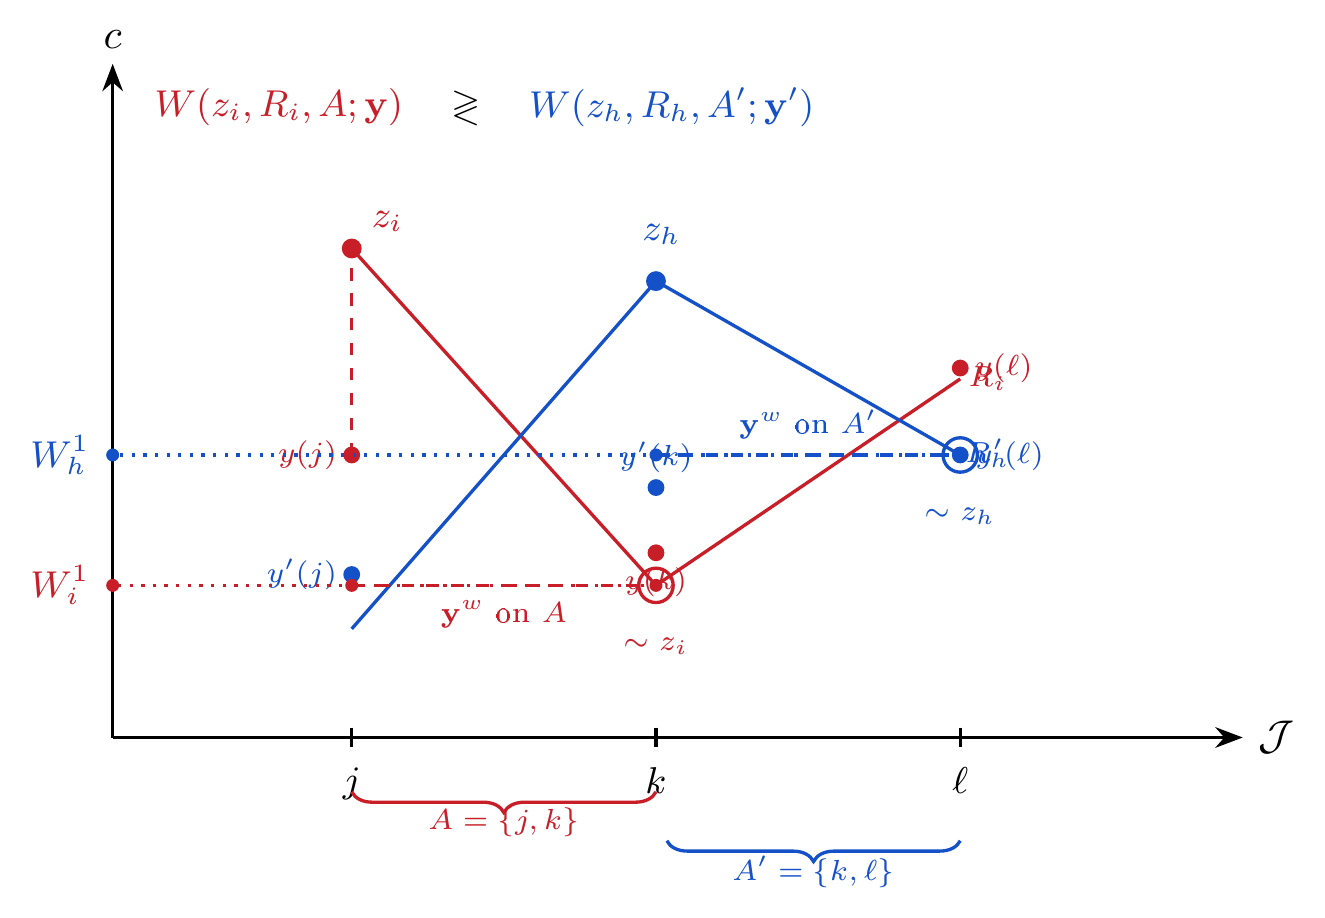
\includegraphics[height=0.57\textheight,width=\textwidth,keepaspectratio]{theory_w1.png}
\end{center}
{\footnotesize Own-set equal-consumption equivalents: each individual gets a common consumption on every job in their own ability set; the level at which the preferred job is indifferent to the attained bundle is their money metric, comparable across individuals. Adapted from Haydar and Maniquet (2026), work in progress.\par}
\cornerlinks{\golink{b:attderiv}{ATT derivation} \golink{b:eaderiv}{EA derivation} \golink{b:prospectref}{prospect reference}}
\note{Estimated utility is not an interpersonal welfare index, because preferences
differ. Each situation is translated into euros through an indifference condition
with an explicit reference, and the choice of reference is the welfare question.

Both money metrics descend from this construction in the companion theory paper:
give every job in a person's own set the same consumption, and find the level at
which the preferred job is exactly as good as the attained bundle. The next two
slides take the construction to the data in two ways: attained outcomes, and job
prospects.}
\end{frame}

% ==================================================================== EA
\begin{frame}
\frametitle{Ex-ante prospect welfare}
\hypertarget{main:ea}{}
\begin{center}
\emph{What constant consumption over the household's own job environment is equivalent to its prospect?}
\end{center}
\slideeq{$\displaystyle\begin{gathered}
  J_i=\int e^{L_i(j)}\Big(\tfrac{C_i(j)}{\lambda_c}\Big)^{\beta_c}\,\widehat g_i(j)\,d\nu(j),
  \qquad
  H_i=\int e^{L_i(j)}\,\widehat g_i(j)\,d\nu(j),
  \\[0.35em]
  M^{\mathrm{EA}}_i=\lambda_c\exp\!\Big\{\tfrac{\log J_i-\log H_i}{\beta_c}\Big\}
  \end{gathered}$}
\begin{columns}[T,onlytextwidth]
\column{0.31\textwidth}\centering
$J_i$\\ {\footnotesize the actual prospect}
\column{0.31\textwidth}\centering
$H_i$\\ {\footnotesize same jobs, equal pay}
\column{0.31\textwidth}\centering
$M^{\mathrm{EA}}_i$\\ {\footnotesize flat-consumption equivalent}
\end{columns}
\vfill
\cornerlinks{\golink{b:eaderiv}{derivation} \golink{b:prospectref}{reference and generalised mean} \golink{b:eavalid}{numerical validation}}
\note{In words: EA is the constant monthly consumption at which a prospect with the
household's own jobs and availability, but equal pay everywhere, is worth exactly
as much as the prospect it actually faces.

Every job enters J weighted by how available it is and how much it is valued; H
keeps the same jobs, availability and preferences with pay differences removed.
Opportunities enter welfare directly: access moves which jobs carry weight, and
earning opportunities move what they pay. I show this perspective first because
the talk is about opportunities.}
\end{frame}

% ==================================================================== ATT
\begin{frame}
\frametitle{Attained-bundle welfare}
\hypertarget{main:att}{}
\begin{center}
\emph{What is the money equivalent of the attained bundle?}
\end{center}
\slideeq{$\displaystyle M^{\mathrm{att}}_i=C^{\mathrm{obs}}_i\exp\!\left\{\frac{L_i(j^{\mathrm{obs}}_i)-L_i(o)}{\beta_c}\right\}$}
\begin{columns}[T,onlytextwidth]
\column{0.46\textwidth}\centering
$o$\\ {\footnotesize non-employment, reachable by all}
\column{0.46\textwidth}\centering
$j^{\mathrm{obs}}_i$\\ {\footnotesize the only route for opportunities}
\end{columns}
\vfill
\cornerlinks{\golink{b:attderiv}{derivation} \golink{b:attdesign}{numerical design}}
\note{In words: ATT is observed consumption, adjusted by the leisure the job costs
relative to not working, converted at the rate one over the consumption weight.

The reference is non-employment, which every household can reach; on the
estimated domain it is also the equal-pay preferred job for every household, so
the measure is the staying-home equivalent. Opportunities matter through which job
is attained and what it pays.

The two measures answer different welfare questions: attained outcomes versus job
prospects. Neither corrects the other.}
\end{frame}

% ==================================================================== Shapley
\begin{frame}
\frametitle{Inequality and Shapley decomposition}
\hypertarget{main:shapley}{}
\vfill
\begin{columns}[T,onlytextwidth]
\column{0.23\textwidth}\centering
\textcolor{chpref}{\textbf{P}}\\ {\footnotesize preferences: age, children}
\column{0.23\textwidth}\centering
\textcolor{chacc}{\textbf{A}}\\ {\footnotesize local unemployment exposure, region, urban or rural location, year}
\column{0.23\textwidth}\centering
\textcolor{chearn}{\textbf{B}}\\ {\footnotesize wage-offer location}
\column{0.23\textwidth}\centering
\textcolor{chneeds}{\textbf{held fixed}}\\ {\footnotesize household resources, needs and composition}
\end{columns}
\slideeq{$\displaystyle\phi^p_k=\sum_{S\subseteq\{P,A,B\}\setminus\{k\}}\frac{|S|!\,(3-|S|-1)!}{3!}\Big[v^p(S\cup\{k\})-v^p(S)\Big]$}
\begin{center}
$v^p(S)=I^p(\varnothing)-I^p(S)$ \qquad $I^p$: household-weighted Gini of $M^p$
\end{center}
\vfill
\cornerlinks{\golink{b:shapley}{Shapley vs one-factor} \golink{b:eagini}{full tables}}
\note{In words: a channel's Shapley contribution is its marginal effect on
inequality, averaged over every order in which the three equalisations can be
introduced; the three contributions add up exactly to the total change.

P equalises age profiles and the child-related shifter. A equalises local access:
local unemployment exposure, region, urban or rural location, and year. B
equalises the systematic wage-offer location. Household resources, needs and
composition are held fixed in every coalition. Each coalition is a full structural
counterfactual: coefficients never change, welfare is recomputed for every
household under each perspective, and inequality is measured again.}
\end{frame}

% ==================================================================== how much
\begin{frame}
\frametitle{How much is associated with opportunities?}
\hypertarget{main:howmuch}{}
\vspace{0.2em}
\begin{center}
\renewcommand{\arraystretch}{1.05}
\begin{tabular}{>{\raggedright\arraybackslash}p{0.34\textwidth}>{\centering\arraybackslash}p{0.22\textwidth}>{\centering\arraybackslash}p{0.22\textwidth}}
 & \textbf{Single adults} & \textbf{Couples} \\[0.2em]
\textcolor{chacc}{\textbf{Ex-ante prospect}}\newline{\small equivalised} & {\huge \VEASingOppEq\%} & {\huge \VEACoupOppEq\%} \\
 & {\color{gray}\scriptsize raw \VEASingOppRaw\%} & {\color{gray}\scriptsize raw \VEACoupOppRaw\%} \\[0.5em]
\textcolor{chearn}{\textbf{Attained bundle}}\newline{\small equivalised} & {\huge \VAttSingOppEq\%} & {\huge \VAttCoupOppEq\%} \\
 & {\color{gray}\scriptsize raw \VAttSingOppRaw\%} & {\color{gray}\scriptsize raw \VAttCoupOppRaw\%} \\
\end{tabular}
\end{center}
\vfill
\begin{center}
\textbf{A + B as \% of the relevant baseline Gini}
\end{center}
\vfill
\cornerlinks{\golink{b:eagini}{EA decomposition} \golink{b:attgini}{ATT decomposition} \golink{b:equiv}{equivalisation} \golink{b:central}{figure}}
\note{The headline. Each number is local access plus earning opportunities as a
percentage of that perspective's own baseline Gini, on the equivalised scale.

Under prospect welfare, the two opportunity channels account for \VEASingOppEq{}
per cent of baseline welfare inequality for single adults and \VEACoupOppEq{} per
cent for couples. Under attained-bundle welfare they account for \VAttSingOppEq{}
and \VAttCoupOppEq{} per cent. The small grey numbers are the raw household scale.

The ATT calculation is the less numerically mature of the two and is a useful
benchmark rather than the sole basis of the paper.}
\end{frame}

% ==================================================================== which channel
\begin{frame}
\frametitle{Which opportunity channel matters?}
\hypertarget{main:channel}{}
\vfill
\begin{columns}[T,onlytextwidth]
\column{0.46\textwidth}
\centering
\textbf{Single adults}\\[0.6em]
{\small\textcolor{chacc}{access}}\\
{\Huge \VChEASingAEq\%}\\[0.5em]
{\small\textcolor{chearn}{earning opportunities}}\\
{\Huge \VChEASingBEq\%}\\[0.5em]
{\small A + B $=$ \VEASingOppEq\%}
\column{0.46\textwidth}
\centering
\textbf{Couples}\\[0.6em]
{\small\textcolor{chacc}{access}}\\
{\Huge \VChEACoupAEq\%}\\[0.5em]
{\small\textcolor{chearn}{earning opportunities}}\\
{\Huge \VChEACoupBEq\%}\\[0.5em]
{\small A + B $=$ \VEACoupOppEq\%}
\end{columns}
\vfill
\begin{center}
{\small prospect welfare, equivalised: \% of baseline Gini}\\[0.3em]
single adults: access $>$ earnings \qquad couples: earnings $>$ access\\[0.3em]
{\small attained-bundle welfare: earnings $>$ access for both populations}
\end{center}
\cornerlinks{\golink{b:eapct}{EA channels} \golink{b:attpct}{ATT channels}}
\note{Now split the prospect-welfare number into its two channels, each as a
percentage of the baseline Gini on the equivalised scale.

Under prospect welfare, access contributes more than earning opportunities for
single adults; for couples, earning opportunities contribute more than access.
Under attained-bundle welfare the ordering for single adults is reversed: earning
opportunities are larger than access for both populations. The full tables, with
Gini points and the raw scale, are one click away.}
\end{frame}

% ==================================================================== 100 per cent
\begin{frame}
\frametitle{Where does baseline inequality go?}
\hypertarget{main:hundred}{}
{\scriptsize\color{gray} shares of baseline Gini \ $\cdot$\ prospect welfare, equivalised\par}
\vfill
\begin{center}\small
\renewcommand{\arraystretch}{1.15}
\begin{tabular}{>{\raggedright\arraybackslash}p{0.62\textwidth}rr}
\toprule
 & \textbf{Single adults} & \textbf{Couples} \\
\midrule
\textcolor{chpref}{Preferences} \quad $\phi_P/I_0$ & \VHundredSingP\% & \VHundredCoupP\% \\
\textcolor{chacc}{Local access} \quad $\phi_A/I_0$ & \VHundredSingA\% & \VHundredCoupA\% \\
\textcolor{chearn}{Earning opportunities} \quad $\phi_B/I_0$ & \VHundredSingB\% & \VHundredCoupB\% \\
\textbf{Other / outside current P-A-B decomposition} \quad $1-(\phi_P+\phi_A+\phi_B)/I_0$ & \VHundredSingRest\% & \VHundredCoupRest\% \\
\midrule
Total & \VHundredSingTotal\% & \VHundredCoupTotal\% \\
\bottomrule
\end{tabular}
\end{center}
\vfill
{\scriptsize Couples: A + B alone $=$ \VHundredCoupAB\%; P + A + B $=$ \VHundredCoupExplained\% because the preference contribution is negative (\VHundredCoupP\%).\par}
\vspace{0.3em}
{\tiny\color{gray} Current decomposition equalises P, A and B only.\par}
\vspace{1.0em}
\cornerlinks{\golink{b:eapct}{channels in Gini points} \golink{b:residual}{outside P-A-B}}
\note{The same prospect-welfare decomposition, laid out so that it visibly sums to
the whole baseline Gini on the equivalised scale.

Under the current ex-ante decomposition, labour-market opportunities account for
about \VHundredSingAB{} per cent of baseline welfare inequality for single adults
and about \VHundredCoupAB{} per cent for couples.

For couples the preference contribution is negative, so preferences plus access
plus earnings is smaller than access plus earnings alone. The last row is
everything the current decomposition does not equalise; what it contains is in the
backup.}
\end{frame}

% ==================================================================== scope
\begin{frame}
\frametitle{What is not claimed}
\hypertarget{main:limits}{}
\vfill
\begin{columns}[T,onlytextwidth]
\column{0.46\textwidth}
\centering
\textbf{Scope}\\[0.6em]
{\small Household resources, needs and composition held fixed}\\[0.5em]
{\small Access: local access, not total opportunity}\\[0.5em]
{\small Preliminary decomposition}
\column{0.46\textwidth}
\centering
\textbf{Not claimed}\\[0.6em]
{\small Not causal}\\[0.5em]
{\small No parameter uncertainty yet}\\[0.5em]
{\small Preferences are not responsibility}\\[0.5em]
{\small Neither perspective is designated primary}
\end{columns}
\vfill
\begin{center}
{\small prospects versus attained outcomes: two different welfare questions}
\end{center}
\vfill
\cornerlinks{\golink{b:residual}{outside P-A-B} \golink{b:uncertainty}{parameter uncertainty} \golink{b:robust}{robustness}}
\note{The scope, stated once.

The decomposition equalises preferences, local access and earning opportunities,
and holds household resources, needs and composition fixed. Access is local
access, not total opportunity. It is a structural accounting exercise, not a
causal decomposition, and parameter uncertainty has not yet been propagated
through it. The preference channel is not a responsibility channel: it contains a
reduced-form child term that can capture constraints as well as tastes. And the
two welfare perspectives answer different questions; choosing between them is a
normative decision not made here.}
\end{frame}

% ==================================================================== conclusion
\begin{frame}
\frametitle{Conclusion}
\hypertarget{main:conclusion}{}
\vfill
\begin{enumerate}\itemsep0.9em
  \item Choices reflect opportunities, not preferences alone.
  \item Prospects: access leads for single adults.\quad Attained outcomes: earnings lead.\quad Couples: earnings lead under both.
  \item Opportunities account for a bounded part of welfare inequality; the preference contribution changes sign with equivalisation.
\end{enumerate}
\vfill
\begin{center}
{\small Next: extend the decomposition to household resources and needs.}
\end{center}
\vfill
\cornerlinks{\golink{main:limits}{scope} \golink{b:residual}{next steps} \golink{appmap}{appendix map}}
\note{Three answers.

First, observed choices carry information about opportunities: a model that gives
everyone the same jobs fits worse on the same households.

Second, the welfare question changes which labour-market inequality matters.
Under prospect welfare, access leads for single adults; under attained-bundle
welfare, earning opportunities lead; for couples, earning opportunities lead under
both.

Third, local access and earning opportunities account for a bounded part of
welfare inequality, and the preference contribution changes sign with
equivalisation.

Next: extend the decomposition to household resources and needs, after fixing the
appropriate operator. Thank you.}
\end{frame}

% ============================================================ BACKUP
\appendix

% ==================================================================== map
\begin{frame}
\frametitle{Appendix map}
\hypertarget{appmap}{}
\vfill
\begin{center}\scriptsize
\renewcommand{\arraystretch}{1.5}
\setlength{\tabcolsep}{4pt}
\begin{tabular}{>{\bfseries}l llll}
Literature & \maplink{b:eopbench}{EOp benchmarks} & \maplink{b:lit}{Literature} & & \\
Model & \maplink{b:utility}{Utility specification} & \maplink{b:density}{Opportunity density} & \maplink{b:likelihood}{Likelihood} & \maplink{b:ident}{Identification} \\
 & \maplink{b:obseq}{Observational equivalence} & & & \\
Estimation & \maplink{b:prefs}{Preferences} & \maplink{b:access}{Employment access} & \maplink{b:hours}{Hours and occupation} & \maplink{b:wage}{Wage offers} \\
 & \maplink{b:benchmarks}{Common opportunities} & \maplink{b:inference}{Inference} & \maplink{b:uncertainty}{Parameter uncertainty} & \\
Fit & \maplink{b:extensive}{Extensive margin} & \maplink{b:margins}{Fit by margin} & \maplink{b:hours37}{Thirty-seven-hour point} & \maplink{b:matched}{Matched households} \\
 & \maplink{b:mrs}{Marginal rate of substitution} & & & \\
Welfare & \maplink{b:attderiv}{ATT derivation} & \maplink{b:eaderiv}{EA derivation} & \maplink{b:eavalid}{EA validation} & \maplink{b:equiv}{Equivalisation} \\
 & \maplink{b:prospectref}{Prospect reference} & \maplink{b:attdesign}{ATT numerical design} & & \\
Decomposition & \maplink{b:central}{Central figure} & \maplink{b:eagini}{EA Gini points} & \maplink{b:attgini}{ATT Gini points} & \maplink{b:eapct}{EA channel shares} \\
 & \maplink{b:attpct}{ATT channel shares} & \maplink{b:explained}{Composition within P/A/B} & \maplink{b:shapley}{Shapley vs one-factor} & \maplink{b:residual}{Outside P-A-B} \\
 & \maplink{b:robust}{Robustness} & & & \\
Data & \maplink{b:sample}{Sample selection} & \maplink{b:pricing}{EUROMOD pricing} & \maplink{b:numerics}{Numerical design} & \\
\end{tabular}
\end{center}
\vfill
\cornerlinks{\hyperlink{main:conclusion}{\beamerreturnbutton{Back}}}
\note{The appendix map. Every entry is a link; every backup slide has a Back
button to the main slide it supports and a button back to this map.}
\end{frame}

% ==================================================================== V19 LITERATURE BACKUPS
\begin{frame}
\frametitle{Backup: inequality-of-opportunity benchmarks}
\hypertarget{b:eopbench}{}
\vfill
\begin{center}\scriptsize
\renewcommand{\arraystretch}{1.35}
\setlength{\tabcolsep}{4pt}
\begin{tabular}{lcll>{\raggedright\arraybackslash}p{0.17\textwidth}>{\raggedright\arraybackslash}p{0.2\textwidth}}
\toprule
 & share & outcome & data & measure & source \\
\midrule
Italy & \VLitItaly\% & gross earnings & \VLitItalyData & MLD; parental education & Checchi \& Peragine (\VLitItalyYear), \VLitItalyWhere \\
Brazil, urban & \VLitBrazilLo--\VLitBrazilHi\% & male hourly earnings & \VLitBrazilData & Theil; five circumstances & Bourguignon et al.\ (\VLitBrazilYear), abstract \\
France & \VLitFrance\% & post-tax earnings & \VLitFranceData & MLD; five circumstances & Brunori et al.\ (\VLitFranceYear), \VLitFranceWhere{} \\
\bottomrule
\end{tabular}
\end{center}
\vfill
\begin{columns}[T,onlytextwidth]
\column{0.48\textwidth}\centering
\textbf{These benchmarks}\\ {\footnotesize shares of earnings inequality attributed to observed circumstances}
\column{0.48\textwidth}\centering
\textbf{This paper}\\ {\footnotesize a share of welfare inequality from estimated latent opportunity components, resources and needs held fixed}
\end{columns}
\vfill
\backnav{main:eop}
\note{Full citations. Checchi and Peragine, Inequality of opportunity in Italy,
Journal of Economic Inequality: the Italy share is in their decomposition table and text. Bourguignon,
Ferreira and Men\'endez, Inequality of opportunity in Brazil, Review of Income and
Wealth: the range is stated in the abstract and conclusion. Brunori, Ferreira and
Peragine, Inequality of opportunity, income inequality and economic mobility, IZA
Discussion Paper: France is in their cross-country table, which reports the estimate of Checchi,
Peragine and Serlenga; that primary study is not in our corpus.

Comparability. These estimates are lower-bound shares of earnings or income
inequality attributed to observed circumstances: adding circumstances can only
raise them. This paper's share is a share of welfare inequality associated with
estimated latent opportunity components, with household resources and needs held
fixed. The outcomes, the circumstance sets and the methods all differ, so the
numbers orient the audience rather than rank countries or papers.}
\end{frame}

\begin{frame}
\frametitle{Backup: literature}
\hypertarget{b:lit}{}
\vfill
\begin{columns}[T,onlytextwidth]
\column{0.31\textwidth}\centering
\textbf{Choice sets and restrictions}\\[0.4em]
{\footnotesize Aaberge, Colombino \& Wennemo (\VLitAcwYear): alternative representations of the choice set}\\[0.3em]
{\footnotesize Beffy, Blundell, Bozio, Laroque \& T\^o (\VLitBeffyYear): labour supply with restricted choices}
\column{0.31\textwidth}\centering
\textbf{Latent jobs and welfare}\\[0.4em]
{\footnotesize Aaberge, Dagsvik \& Str{\o}m; Dagsvik \& Str{\o}m; Dagsvik \& Jia; Cap\'eau, Decoster \& Dekkers}\\[0.3em]
{\footnotesize Fleurbaey \& Maniquet; Decoster \& Haan; Bargain et al.; Jacquet, Jia \& Thoresen}
\column{0.31\textwidth}\centering
\textbf{Inequality of opportunity and decomposition}\\[0.4em]
{\footnotesize Roemer; Checchi \& Peragine; Bourguignon, Ferreira \& Men\'endez; Brunori, Ferreira \& Peragine}\\[0.3em]
{\footnotesize Shorrocks; Sastre \& Trannoy; Creedy \& H\'erault; M\"uhlhan}
\end{columns}
\vfill
\backnav{main:blocks}
\note{Two papers matter most for separating preferences from opportunities.
Aaberge, Colombino and Wennemo compare alternative representations of the choice
set in labour-supply models, which is exactly the object our opportunity density
replaces with an estimated one. Beffy, Blundell, Bozio, Laroque and T\^o model
labour supply with restricted choices, the same concern that hours opportunities
are not freely chosen. The other columns list the latent-jobs, welfare,
inequality-of-opportunity and decomposition references behind the main slides.}
\end{frame}

\begin{frame}
\frametitle{Backup: observational equivalence}
\hypertarget{b:obseq}{}
\vfill
\begin{columns}[T,onlytextwidth]
\column{0.46\textwidth}\centering
\textbf{Without restrictions}\\[0.4em]
{\small a taste against certain hours and a scarcity of jobs at those hours predict the same choices}
\column{0.46\textwidth}\centering
\textbf{With restrictions}\\[0.4em]
{\small smooth tastes, banded availability and excluded access shifters move different parts of the choice distribution}
\end{columns}
\vfill
\begin{center}
If availability heterogeneity is omitted, some of its effects can be absorbed by the estimated utility component.
\end{center}
\vfill
\begin{center}
{\small maintained restrictions, not tested \quad$\cdot$\quad regional variation is not a causal design}
\end{center}
\vfill
\backnav{main:ident}
\note{Choices alone do not separate a taste for leisure from a scarcity of jobs at
that number of hours: the two can be observationally equivalent. The separation
comes from maintained functional-form and exclusion restrictions: smooth
preferences against banded hours opportunities, access shifters excluded from
utility, and wage offers independent of hours given occupation. If availability
heterogeneity is omitted, some of its effects can be absorbed by the estimated
utility component. These restrictions are maintained rather than tested, and the
regional variation supports the access block only conditional on them.}
\end{frame}

\begin{frame}
\frametitle{Backup: attained-bundle numerical design}
\hypertarget{b:attdesign}{}
\vfill
\begin{columns}[T,onlytextwidth]
\column{0.31\textwidth}\centering
\textbf{Sample}\\[0.4em]
{\footnotesize the already-priced estimation panel; no re-estimation and no new pricing}
\column{0.31\textwidth}\centering
\textbf{Counterfactuals}\\[0.4em]
{\footnotesize equalised covariates set to household-weighted means; attained bundle simulated by Gumbel-max with common random numbers}
\column{0.31\textwidth}\centering
\textbf{Checks}\\[0.4em]
{\footnotesize replications at fixed estimates; an independent second seed; exact Shapley closure}
\end{columns}
\vfill
\begin{center}
{\small short weekly hours are sparsely represented in the integration panel}\\[0.3em]
{\small Monte Carlo ranges are simulation spreads, not confidence intervals}
\end{center}
\vfill
\backnav{main:att}
\note{How the attained-bundle decomposition is computed. It reuses the
already-priced estimation panel. In each coalition the household-constant
covariates of the equalised channels are replaced by household-weighted means,
and each household's attained bundle is simulated with the Gumbel-max rule under
common random numbers, so realised taste draws carry through every coalition. The
money metric and the Gini are recomputed, and each coalition value averages many
replications at fixed estimates. An independent second seed reproduces the
allocation, which closes exactly. The main open issue is that the panel
represents short weekly hours sparsely; the effect of that on the attribution has
not been fully quantified, which is why this calculation is still being
validated.}
\end{frame}

\begin{frame}
\frametitle{Backup: the prospect reference}
\hypertarget{b:prospectref}{}
\vfill
\backupeq{$\displaystyle M^{\mathrm{EA}}_i=\Big(\int C_i(j)^{\beta_c}\,\omega_i(j)\,d\nu(j)\Big)^{1/\beta_c},
\qquad \omega_i(j)=\frac{e^{L_i(j)}\,\widehat g_i(j)}{H_i}$}
\vfill
\begin{columns}[T,onlytextwidth]
\column{0.46\textwidth}\centering
\textbf{Own-opportunity reference}\\[0.4em]
{\small the reference prospect keeps the household's own jobs, availability and preferences, and equalises pay}
\column{0.46\textwidth}\centering
\textbf{Weighted generalised mean}\\[0.4em]
{\small the metric is a generalised mean of consumption with exponent $\beta_c$, weighted by leisure value and availability}
\end{columns}
\vfill
\begin{center}
{\small the reference moves with the household's opportunity environment}
\end{center}
\vfill
\backnav{main:ea}
\note{Two readings of the ex-ante metric. First, its reference is the household's
own opportunity environment with pay equalised, so the reference itself moves when
opportunities change: equalising access changes both J and H. Second, dividing J
by H shows that the metric is a weighted generalised mean of consumption across jobs,
with exponent the consumption weight and weights proportional to the leisure value
of each job times its availability. A common rescaling of the density cancels from
those weights. Whether the metric is monotone in opportunity expansions is a
separate question, not discussed in the main talk.}
\end{frame}

\begin{frame}
\frametitle{Backup: parameter uncertainty}
\hypertarget{b:uncertainty}{}
\vfill
\begin{columns}[T,onlytextwidth]
\column{0.31\textwidth}\centering
\textbf{Estimated}\\[0.4em]
{\footnotesize cluster-robust standard errors for every estimated coordinate, clustered on the household}
\column{0.31\textwidth}\centering
\textbf{Not yet propagated}\\[0.4em]
{\footnotesize estimation uncertainty has not been carried through either welfare decomposition}
\column{0.31\textwidth}\centering
\textbf{Simulation checks}\\[0.4em]
{\footnotesize second seeds and repeat runs measure numerical noise, not sampling uncertainty}
\end{columns}
\vfill
\begin{center}
{\small the decomposition shares are point estimates without confidence intervals}
\end{center}
\vfill
\backnav{main:limits}
\note{What is and is not known about uncertainty. Every estimated coordinate has a
cluster-robust standard error. Estimation uncertainty has not been propagated
through either decomposition, so the shares on the result slides are point
estimates without confidence intervals, and differences between them are not
statistically established. The seed and repeat-run comparisons measure numerical
noise in the calculation, not sampling uncertainty. Propagating parameter
uncertainty is a next step.}
\end{frame}

% ==================================================================== MODEL
\begin{frame}
\frametitle{Backup: utility specification}
\hypertarget{b:utility}{}
\vfill
\backupeq{$\displaystyle v_i(j)=L_i(j)+\beta_c\log\!\Big(\frac{C_i(j)}{\lambda_c}\Big),\qquad
L_i(j)=\beta^g_\ell(\mathbf x_i)\,\mathcal B\big(\tilde\ell_i(j);\theta^g_\ell\big)$}
\backupeq{$\displaystyle \tilde\ell_i(j)=\frac{\VTimeEndow-h}{\VLeisureScale},\qquad \mathcal B(z;\theta)=\frac{z^\theta-1}{\theta}$}
\vfill
\begin{columns}[T,onlytextwidth]
\column{0.31\textwidth}\centering
$\beta^g_\ell(\mathbf x_i)$\\ {\footnotesize intercept, centred age and its square (units of \VAgeScale{} years)}
\column{0.31\textwidth}\centering
$k_i$\\ {\footnotesize children under \VChildCutoff, women only}
\column{0.31\textwidth}\centering
couples\\ {\footnotesize sum of the two spouses' leisure terms}
\end{columns}
\vfill
\backnav{main:jobs}
\note{The full systematic utility. Leisure is weekly time left from a maintained
endowment, rescaled, and passed through a Box-Cox transform with a group-specific
curvature. The leisure weight varies with centred age and, for women, with the
number of children; that child term is a reduced-form time-constraint shifter,
not pure taste. The consumption weight is estimated. The shock is extreme value
with unit scale.}
\end{frame}

\begin{frame}
\frametitle{Backup: opportunity density}
\hypertarget{b:density}{}
\vfill
\backupeq{$\displaystyle g_i(o)=1,\qquad g_i(j)=g^{E}_i\;g^{H}_i(h)\;g^{\mathrm{Occ}}_i(k)\;g^{W}_i(w\mid k)\quad\text{for market jobs } j\neq o$}
\vfill
\begin{columns}[T,onlytextwidth]
\column{0.23\textwidth}\centering
\textcolor{chacc}{\textbf{access}}\\ {\footnotesize $g^E_i$: local unemployment exposure, region, urban or rural location, year}
\column{0.23\textwidth}\centering
\textbf{hours}\\ {\footnotesize $g^H_i$: elevated bands over a residual set}
\column{0.23\textwidth}\centering
\textbf{occupation}\\ {\footnotesize $g^{\mathrm{Occ}}_i$: sex-specific group masses}
\column{0.23\textwidth}\centering
\textcolor{chearn}{\textbf{wage offers}}\\ {\footnotesize $g^W_i$: log-normal, truncated to $[\VWageLo,\VWageHi]$}
\end{columns}
\vfill
\begin{center}
{\small wage-offer location $\mu_i(k)$: education, potential experience and its square, occupation}
\end{center}
\vfill
\backnav{main:opp}
\note{Non-employment is the reference state with density one. Every market job
carries access, the employment mass, times hours, occupation and wage-offer
factors; for couples, each employed spouse's package carries its own factors.
This is the form of the executed criterion, where the access index multiplies the
working indicator. The
unemployment exposure enters access scaled by \VGsurScale. The wage location
depends on education, potential experience in units of \VExpScale{} years and
occupation, with a common dispersion. The hours density is a density elevation
over intervals, not an atom at a particular hour.}
\end{frame}

\begin{frame}
\frametitle{Backup: sampled-alternative likelihood}
\hypertarget{b:likelihood}{}
\vfill
\backupeq{$\displaystyle V_{ij}=v_i(j)+\log g_i(j)-\log q_{ij}$}
\backupeq{$\displaystyle \Pr\!\big(y\mid\mathcal C_i\big)=\frac{n_y\exp V_{iy}}{\sum_{s\in\mathcal C_i}\exp V_{is}}$}
\vfill
\begin{columns}[T,onlytextwidth]
\column{0.31\textwidth}\centering
$q_{ij}$\\ {\footnotesize proposal density, fitted out of fold}
\column{0.31\textwidth}\centering
$\mathcal C_i$\\ {\footnotesize observed job and \VNDraws{} draws: \VNAltRows{} rows}
\column{0.31\textwidth}\centering
$n_y$\\ {\footnotesize multiplicity of a repeated draw}
\end{columns}
\vfill
\backnav{main:opp}
\note{The choice set is a continuum, so the likelihood is evaluated over sampled
alternatives drawn from a proposal density and corrected by it. The proposal is a
computational device: fitted out of fold so a household's own outcome never
enters the proposal used to score it, and it enters no welfare measure. For
couples the proposal draws the joint participation regime first.}
\end{frame}

\begin{frame}
\frametitle{Backup: identification}
\hypertarget{b:ident}{}
\vfill
\begin{columns}[T,onlytextwidth]
\column{0.31\textwidth}\centering
\textbf{Functional form}\\[0.4em]
{\footnotesize smooth preferences in hours; banded hours opportunities}
\column{0.31\textwidth}\centering
\textbf{Exclusion}\\[0.4em]
{\footnotesize local unemployment exposure and geography shift access, not utility}
\column{0.31\textwidth}\centering
\textbf{Independence}\\[0.4em]
{\footnotesize wage offers independent of hours, given occupation}
\end{columns}
\vfill
\begin{center}
{\small maintained, not tested \quad$\cdot$\quad not a causal design}
\end{center}
\vfill
\backnav{main:ident}
\note{Choices alone do not separate a taste for leisure from a scarcity of jobs at
that number of hours. Three restrictions do the work: a spike at a band of hours
is read as availability rather than a kink in tastes; excluded shifters enter
availability and not preferences; and wage offers are independent of hours given
occupation. These are the restrictions of the latent-jobs literature, maintained
here rather than tested. No causal effect of geography is claimed.}
\end{frame}

% ==================================================================== ESTIMATION
\begin{frame}
\frametitle{Backup: preference parameters}
\hypertarget{b:prefs}{}
\vfill
\begin{center}\scriptsize
\renewcommand{\arraystretch}{1.05}
\setlength{\tabcolsep}{4pt}
\begin{tabular}{lcccc}
\toprule
 & Single men & Single women & Couple men & Couple women \\
\midrule
leisure weight, intercept & \VCoefSingBetaZeroLSm{} \se{\VCoefSingBetaZeroLSmSE} & \VCoefSingBetaZeroLSf{} \se{\VCoefSingBetaZeroLSfSE} & \VCoefCoupBetaZeroLM{} \se{\VCoefCoupBetaZeroLMSE} & \VCoefCoupBetaZeroLF{} \se{\VCoefCoupBetaZeroLFSE} \\
 & {\tiny\color{gray}\VCoefSingBetaZeroLSmId} & {\tiny\color{gray}\VCoefSingBetaZeroLSfId} & {\tiny\color{gray}\VCoefCoupBetaZeroLMId} & {\tiny\color{gray}\VCoefCoupBetaZeroLFId} \\[0.2em]
leisure weight, age & \VCoefSingBetaLAgeSm{} \se{\VCoefSingBetaLAgeSmSE} & \VCoefSingBetaLAgeSf{} \se{\VCoefSingBetaLAgeSfSE} & \VCoefCoupBetaLAgeM{} \se{\VCoefCoupBetaLAgeMSE} & \VCoefCoupBetaLAgeF{} \se{\VCoefCoupBetaLAgeFSE} \\
 & {\tiny\color{gray}\VCoefSingBetaLAgeSmId} & {\tiny\color{gray}\VCoefSingBetaLAgeSfId} & {\tiny\color{gray}\VCoefCoupBetaLAgeMId} & {\tiny\color{gray}\VCoefCoupBetaLAgeFId} \\[0.2em]
leisure weight, age squared & \VCoefSingBetaLTwoAgeSm{} \se{\VCoefSingBetaLTwoAgeSmSE} & \VCoefSingBetaLTwoAgeSf{} \se{\VCoefSingBetaLTwoAgeSfSE} & \VCoefCoupBetaLTwoAgeM{} \se{\VCoefCoupBetaLTwoAgeMSE} & \VCoefCoupBetaLTwoAgeF{} \se{\VCoefCoupBetaLTwoAgeFSE} \\
 & {\tiny\color{gray}\VCoefSingBetaLTwoAgeSmId} & {\tiny\color{gray}\VCoefSingBetaLTwoAgeSfId} & {\tiny\color{gray}\VCoefCoupBetaLTwoAgeMId} & {\tiny\color{gray}\VCoefCoupBetaLTwoAgeFId} \\[0.2em]
leisure weight, children & --- & \VCoefSingBetaLNkidsSf{} \se{\VCoefSingBetaLNkidsSfSE} & --- & \VCoefCoupBetaLNkidsF{} \se{\VCoefCoupBetaLNkidsFSE} \\
 &  & {\tiny\color{gray}\VCoefSingBetaLNkidsSfId} &  & {\tiny\color{gray}\VCoefCoupBetaLNkidsFId} \\[0.2em]
leisure curvature $\theta_\ell$ & \VCoefSingThetaLSm{} \se{\VCoefSingThetaLSmSE} & \VCoefSingThetaLSf{} \se{\VCoefSingThetaLSfSE} & \VCoefCoupThetaLM{} \se{\VCoefCoupThetaLMSE} & \VCoefCoupThetaLF{} \se{\VCoefCoupThetaLFSE} \\
 & {\tiny\color{gray}\VCoefSingThetaLSmId} & {\tiny\color{gray}\VCoefSingThetaLSfId} & {\tiny\color{gray}\VCoefCoupThetaLMId} & {\tiny\color{gray}\VCoefCoupThetaLFId} \\[0.2em]
consumption weight $\beta_c$ & \multicolumn{2}{c}{\VCoefSingBetaC{} \se{\VCoefSingBetaCSE}} & \multicolumn{2}{c}{\VCoefCoupBetaC{} \se{\VCoefCoupBetaCSE}} \\
 & \multicolumn{2}{c}{{\tiny\color{gray}\VCoefSingBetaCId}} & \multicolumn{2}{c}{{\tiny\color{gray}\VCoefCoupBetaCId}} \\
\bottomrule
\end{tabular}
\end{center}
\vfill
{\footnotesize cluster-robust standard errors; parameter identifiers in grey; the male children term in couples is structurally zero}
\backnav{main:sel}
\note{The preference block, with the parameter identifiers used in estimation. The
consumption weight is common within each population. One single-adult coordinate,
the female age-square term, sits at a box endpoint, so its standard error is not
reported and it is excluded from the interior curvature. Levels are not comparable
across the two separately estimated models.}
\end{frame}

\begin{frame}
\frametitle{Backup: employment-access parameters}
\hypertarget{b:access}{}
\vfill
\begin{center}\scriptsize
\renewcommand{\arraystretch}{1.1}
\begin{tabular}{llcc}
\toprule
 & identifier & Singles & Couples \\
\midrule
employment constant & {\tiny\color{gray}\VCoefSingBetaEId; \VCoefCoupBetaEMId, \VCoefCoupBetaEFId} & \VCoefSingBetaE{} \se{\VCoefSingBetaESE} & men \VCoefCoupBetaEM{} \se{\VCoefCoupBetaEMSE} \\
 & & & women \VCoefCoupBetaEF{} \se{\VCoefCoupBetaEFSE} \\
local unemployment exposure & {\tiny\color{gray}\VCoefSingBetaEGsurId} & \VCoefSingBetaEGsur{} \se{\VCoefSingBetaEGsurSE} & \VCoefCoupBetaEGsur{} \se{\VCoefCoupBetaEGsurSE} \\
densely populated & {\tiny\color{gray}\VCoefSingBetaEDrgurId} & \VCoefSingBetaEDrgur{} \se{\VCoefSingBetaEDrgurSE} & \VCoefCoupBetaEDrgur{} \se{\VCoefCoupBetaEDrgurSE} \\
intermediate density & {\tiny\color{gray}\VCoefSingBetaEDrgmdId} & \VCoefSingBetaEDrgmd{} \se{\VCoefSingBetaEDrgmdSE} & \VCoefCoupBetaEDrgmd{} \se{\VCoefCoupBetaEDrgmdSE} \\
\VCoefSingBetaETwoDrgnLabel & {\tiny\color{gray}\VCoefSingBetaETwoDrgnId} & \VCoefSingBetaETwoDrgn{} \se{\VCoefSingBetaETwoDrgnSE} & \VCoefCoupBetaETwoDrgn{} \se{\VCoefCoupBetaETwoDrgnSE} \\
\VCoefSingBetaEThreeDrgnLabel & {\tiny\color{gray}\VCoefSingBetaEThreeDrgnId} & \VCoefSingBetaEThreeDrgn{} \se{\VCoefSingBetaEThreeDrgnSE} & \VCoefCoupBetaEThreeDrgn{} \se{\VCoefCoupBetaEThreeDrgnSE} \\
\VCoefSingBetaEFourDrgnLabel & {\tiny\color{gray}\VCoefSingBetaEFourDrgnId} & \VCoefSingBetaEFourDrgn{} \se{\VCoefSingBetaEFourDrgnSE} & \VCoefCoupBetaEFourDrgn{} \se{\VCoefCoupBetaEFourDrgnSE} \\
\VCoefSingBetaEFiveDrgnLabel & {\tiny\color{gray}\VCoefSingBetaEFiveDrgnId} & \VCoefSingBetaEFiveDrgn{} \se{\VCoefSingBetaEFiveDrgnSE} & \VCoefCoupBetaEFiveDrgn{} \se{\VCoefCoupBetaEFiveDrgnSE} \\
\VCoefSingBetaESixDrgnLabel & {\tiny\color{gray}\VCoefSingBetaESixDrgnId} & \VCoefSingBetaESixDrgn{} \se{\VCoefSingBetaESixDrgnSE} & \VCoefCoupBetaESixDrgn{} \se{\VCoefCoupBetaESixDrgnSE} \\
\VCoefSingBetaESevenDrgnLabel & {\tiny\color{gray}\VCoefSingBetaESevenDrgnId} & \VCoefSingBetaESevenDrgn{} \se{\VCoefSingBetaESevenDrgnSE} & \VCoefCoupBetaESevenDrgn{} \se{\VCoefCoupBetaESevenDrgnSE} \\
\VCoefSingBetaEEightDrgnLabel & {\tiny\color{gray}\VCoefSingBetaEEightDrgnId} & \VCoefSingBetaEEightDrgn{} \se{\VCoefSingBetaEEightDrgnSE} & \VCoefCoupBetaEEightDrgn{} \se{\VCoefCoupBetaEEightDrgnSE} \\
\bottomrule
\end{tabular}
\end{center}
\vfill
{\footnotesize references: the first region and thinly populated areas; couples share the shifters across spouses}
\backnav{main:sel}
\note{The employment-access block of market jobs, with identifiers. The access
index multiplies the working indicator, so non-employment is the reference. Local
unemployment exposure lowers employment opportunity mass in both populations.
Regional and urbanisation indicators shift access conditional on the exclusion
restriction.}
\end{frame}

\begin{frame}
\frametitle{Backup: hours and occupation opportunities}
\hypertarget{b:hours}{}
\vspace{-0.6em}
\begin{center}\scriptsize
\textbf{Hours bands}\\[0.2em]
\renewcommand{\arraystretch}{0.78}
\begin{tabular}{lccc}
\toprule
 & Singles & Couple men & Couple women \\
\midrule
part-time lower & \VCoefSingBetaHOnePt & \VCoefCoupBetaHOnePtM & \VCoefCoupBetaHOnePtF \\
 & {\tiny\color{gray}\VCoefSingBetaHOnePtId} & {\tiny\color{gray}\VCoefCoupBetaHOnePtMId} & {\tiny\color{gray}\VCoefCoupBetaHOnePtFId} \\
part-time upper & \VCoefSingBetaHTwoPt & \VCoefCoupBetaHTwoPtM & \VCoefCoupBetaHTwoPtF \\
 & {\tiny\color{gray}\VCoefSingBetaHTwoPtId} & {\tiny\color{gray}\VCoefCoupBetaHTwoPtMId} & {\tiny\color{gray}\VCoefCoupBetaHTwoPtFId} \\
narrow full-time & \VCoefSingBetaHThreeFiveF & \VCoefCoupBetaHThreeFiveFM & \VCoefCoupBetaHThreeFiveFF \\
 & {\tiny\color{gray}\VCoefSingBetaHThreeFiveFId} & {\tiny\color{gray}\VCoefCoupBetaHThreeFiveFMId} & {\tiny\color{gray}\VCoefCoupBetaHThreeFiveFFId} \\
full-time upper & \VCoefSingBetaHFt & \VCoefCoupBetaHFtM & \VCoefCoupBetaHFtF \\
 & {\tiny\color{gray}\VCoefSingBetaHFtId} & {\tiny\color{gray}\VCoefCoupBetaHFtMId} & {\tiny\color{gray}\VCoefCoupBetaHFtFId} \\
long hours & \VCoefSingBetaHLh & \VCoefCoupBetaHLhM & \VCoefCoupBetaHLhF \\
 & {\tiny\color{gray}\VCoefSingBetaHLhId} & {\tiny\color{gray}\VCoefCoupBetaHLhMId} & {\tiny\color{gray}\VCoefCoupBetaHLhFId} \\
\bottomrule
\end{tabular}\\[0.15em]
\textbf{Occupation masses}\\[0.2em]
\begin{tabular}{lcccc}
\toprule
 & \multicolumn{2}{c}{Singles} & \multicolumn{2}{c}{Couples} \\
 & men & women & men & women \\
\midrule
\VCoefSingBetaOccTwoMLabel & \VCoefSingBetaOccTwoM & \VCoefSingBetaOccTwoF & \VCoefCoupBetaOccTwoM & \VCoefCoupBetaOccTwoF \\
 & {\tiny\color{gray}\VCoefSingBetaOccTwoMId} & {\tiny\color{gray}\VCoefSingBetaOccTwoFId} & {\tiny\color{gray}\VCoefCoupBetaOccTwoMId} & {\tiny\color{gray}\VCoefCoupBetaOccTwoFId} \\
\VCoefSingBetaOccThreeMLabel & \VCoefSingBetaOccThreeM & \VCoefSingBetaOccThreeF & \VCoefCoupBetaOccThreeM & \VCoefCoupBetaOccThreeF \\
 & {\tiny\color{gray}\VCoefSingBetaOccThreeMId} & {\tiny\color{gray}\VCoefSingBetaOccThreeFId} & {\tiny\color{gray}\VCoefCoupBetaOccThreeMId} & {\tiny\color{gray}\VCoefCoupBetaOccThreeFId} \\
\VCoefSingBetaOccFourMLabel & \VCoefSingBetaOccFourM & \VCoefSingBetaOccFourF & \VCoefCoupBetaOccFourM & \VCoefCoupBetaOccFourF \\
 & {\tiny\color{gray}\VCoefSingBetaOccFourMId} & {\tiny\color{gray}\VCoefSingBetaOccFourFId} & {\tiny\color{gray}\VCoefCoupBetaOccFourMId} & {\tiny\color{gray}\VCoefCoupBetaOccFourFId} \\
\bottomrule
\end{tabular}
\end{center}
{\scriptsize estimates with identifiers; standard errors in the paper}
\backnav{main:sel}
\note{Hours opportunities are elevated densities over five bands relative to a
residual set; hours coefficients are common across single men and women and
spouse-specific for couples. Occupation masses are sex-specific, relative to the
craft, agricultural, operator and elementary group. Identifiers are shown under
each estimate.}
\end{frame}

\begin{frame}
\frametitle{Backup: wage-offer equation}
\hypertarget{b:wage}{}
\vfill
\begin{center}\scriptsize
\renewcommand{\arraystretch}{1.2}
\begin{tabular}{llcc}
\toprule
 & identifier & Singles & Couples \\
\midrule
intercept & {\tiny\color{gray}\VCoefSingBetaZeroWId} & \VCoefSingBetaZeroW{} \se{\VCoefSingBetaZeroWSE} & \VCoefCoupBetaZeroW{} \se{\VCoefCoupBetaZeroWSE} \\
low education & {\tiny\color{gray}\VCoefSingBetaWEducLId} & \VCoefSingBetaWEducL{} \se{\VCoefSingBetaWEducLSE} & \VCoefCoupBetaWEducL{} \se{\VCoefCoupBetaWEducLSE} \\
high education & {\tiny\color{gray}\VCoefSingBetaWEducHId} & \VCoefSingBetaWEducH{} \se{\VCoefSingBetaWEducHSE} & \VCoefCoupBetaWEducH{} \se{\VCoefCoupBetaWEducHSE} \\
potential experience & {\tiny\color{gray}\VCoefSingBetaWPexpId} & \VCoefSingBetaWPexp{} \se{\VCoefSingBetaWPexpSE} & \VCoefCoupBetaWPexp{} \se{\VCoefCoupBetaWPexpSE} \\
experience squared & {\tiny\color{gray}\VCoefSingBetaWTwoPexpId} & \VCoefSingBetaWTwoPexp{} \se{\VCoefSingBetaWTwoPexpSE} & \VCoefCoupBetaWTwoPexp{} \se{\VCoefCoupBetaWTwoPexpSE} \\
\VCoefSingDeltaOccTwoLabel & {\tiny\color{gray}\VCoefSingDeltaOccTwoId} & \VCoefSingDeltaOccTwo{} \se{\VCoefSingDeltaOccTwoSE} & \VCoefCoupDeltaOccTwo{} \se{\VCoefCoupDeltaOccTwoSE} \\
\VCoefSingDeltaOccThreeLabel & {\tiny\color{gray}\VCoefSingDeltaOccThreeId} & \VCoefSingDeltaOccThree{} \se{\VCoefSingDeltaOccThreeSE} & \VCoefCoupDeltaOccThree{} \se{\VCoefCoupDeltaOccThreeSE} \\
\VCoefSingDeltaOccFourLabel & {\tiny\color{gray}\VCoefSingDeltaOccFourId} & \VCoefSingDeltaOccFour{} \se{\VCoefSingDeltaOccFourSE} & \VCoefCoupDeltaOccFour{} \se{\VCoefCoupDeltaOccFourSE} \\
log-wage dispersion $\sigma$ & {\tiny\color{gray}\VCoefSingSigmaId} & \VCoefSingSigma{} \se{\VCoefSingSigmaSE} & \VCoefCoupSigma{} \se{\VCoefCoupSigmaSE} \\
\bottomrule
\end{tabular}
\end{center}
\vfill
{\footnotesize medium education is the reference; experience in units of \VExpScale{} years}
\backnav{main:sel}
\note{The wage-offer equation, with identifiers. The offered log wage is normal
with this location and a common dispersion, truncated to the wage support and
renormalised. The singles and couples models are estimated separately, so the two
experience profiles are not restricted to agree.}
\end{frame}

\begin{frame}
\frametitle{Backup: common versus household-specific opportunities}
\hypertarget{b:benchmarks}{}
\vfill
\begin{center}\small
\renewcommand{\arraystretch}{1.35}
\begin{tabular}{>{\raggedright\arraybackslash}p{0.44\textwidth}ccc}
\toprule
Single adults & free coordinates & criterion & population fit \\
\midrule
household-specific opportunities & \VKFreeSingles{} & \VNegllSingles{} & \VMaeSingles{} \\
common opportunity distribution & \VKFreeRumA{} & \VNegllRumA{} & \VMaeRumA{} \\
common shape; employment and hours in utility & \VKFreeRumB{} & \VNegllRumB{} & \VMaeRumB{} \\
\bottomrule
\end{tabular}
\end{center}
\vfill
{\footnotesize same households, sampled alternatives and criterion; not converted into a formal test}
\backnav{main:est}
\note{The two re-estimated common-opportunity benchmarks restrict the opportunity
block and re-estimate everything else. Both are worse on the same criterion, and
population fit worsens where the opportunity block does its work. A better
criterion does not by itself establish that a mechanism has been identified.}
\end{frame}

\begin{frame}
\frametitle{Backup: curvature and inference}
\hypertarget{b:inference}{}
\vfill
\begin{columns}[T,onlytextwidth]
\column{0.46\textwidth}
\centering
\textbf{Single adults}\\[0.5em]
{\small free coordinates \VKFreeSingles{}, interior \VKIntSingles{}}\\
{\small criterion \VNegllSingles{}}\\
{\small smallest Hessian eigenvalue \VMinEigSingles{}}
\column{0.46\textwidth}
\centering
\textbf{Couples}\\[0.5em]
{\small free coordinates \VKFreeCouples{}, interior \VKIntCouples{}}\\
{\small criterion \VNegllCouples{}}\\
{\small smallest Hessian eigenvalue \VMinEigCouples{}}
\end{columns}
\vfill
\begin{center}
{\small cluster-robust standard errors on the household \quad$\cdot$\quad eigenvalues on the interior block}
\end{center}
\vfill
\backnav{main:sel}
\note{Curvature and inference. The exact Hessian on the interior block is
positive definite for both models. Several terminal paths from different starts
agree to numerical precision; that supports a stable local solution from the
starts tested, not global uniqueness. One single-adult coordinate at a box
endpoint is handled under the active-set convention.}
\end{frame}

% ==================================================================== FIT
\begin{frame}
\frametitle{Backup: extensive-margin fit}
\hypertarget{b:extensive}{}
\vfill
\begin{center}\small
\renewcommand{\arraystretch}{1.35}
\begin{tabular}{lccc}
\toprule
 & weighted accuracy & model-simulated range & integration ratio \\
\midrule
single women & \VAccSingleWomen\% & \VAccSingleWomenLo--\VAccSingleWomenHi\% & \VIntRatioSingleWomen \\
coupled women & \VAccCoupledWomen\% & \VAccCoupledWomenLo--\VAccCoupledWomenHi\% & \VIntRatioCoupledWomen \\
single men & withheld & --- & \VIntRatioSingleMen \\
coupled men & withheld & --- & \VIntRatioCoupledMen \\
\bottomrule
\end{tabular}
\end{center}
\vfill
{\footnotesize withheld where numerical integration error is too large relative to sampling variation}
\backnav{main:est}
\note{Extensive-margin accuracy is reportable for women in each sample and
withheld for men, because numerical integration error is too large relative to
sampling variation. The integration ratio is that comparison; the rule was fixed
before the evaluation.}
\end{frame}

\begin{frame}
\frametitle{Backup: fit by margin}
\hypertarget{b:margins}{}
\begin{center}
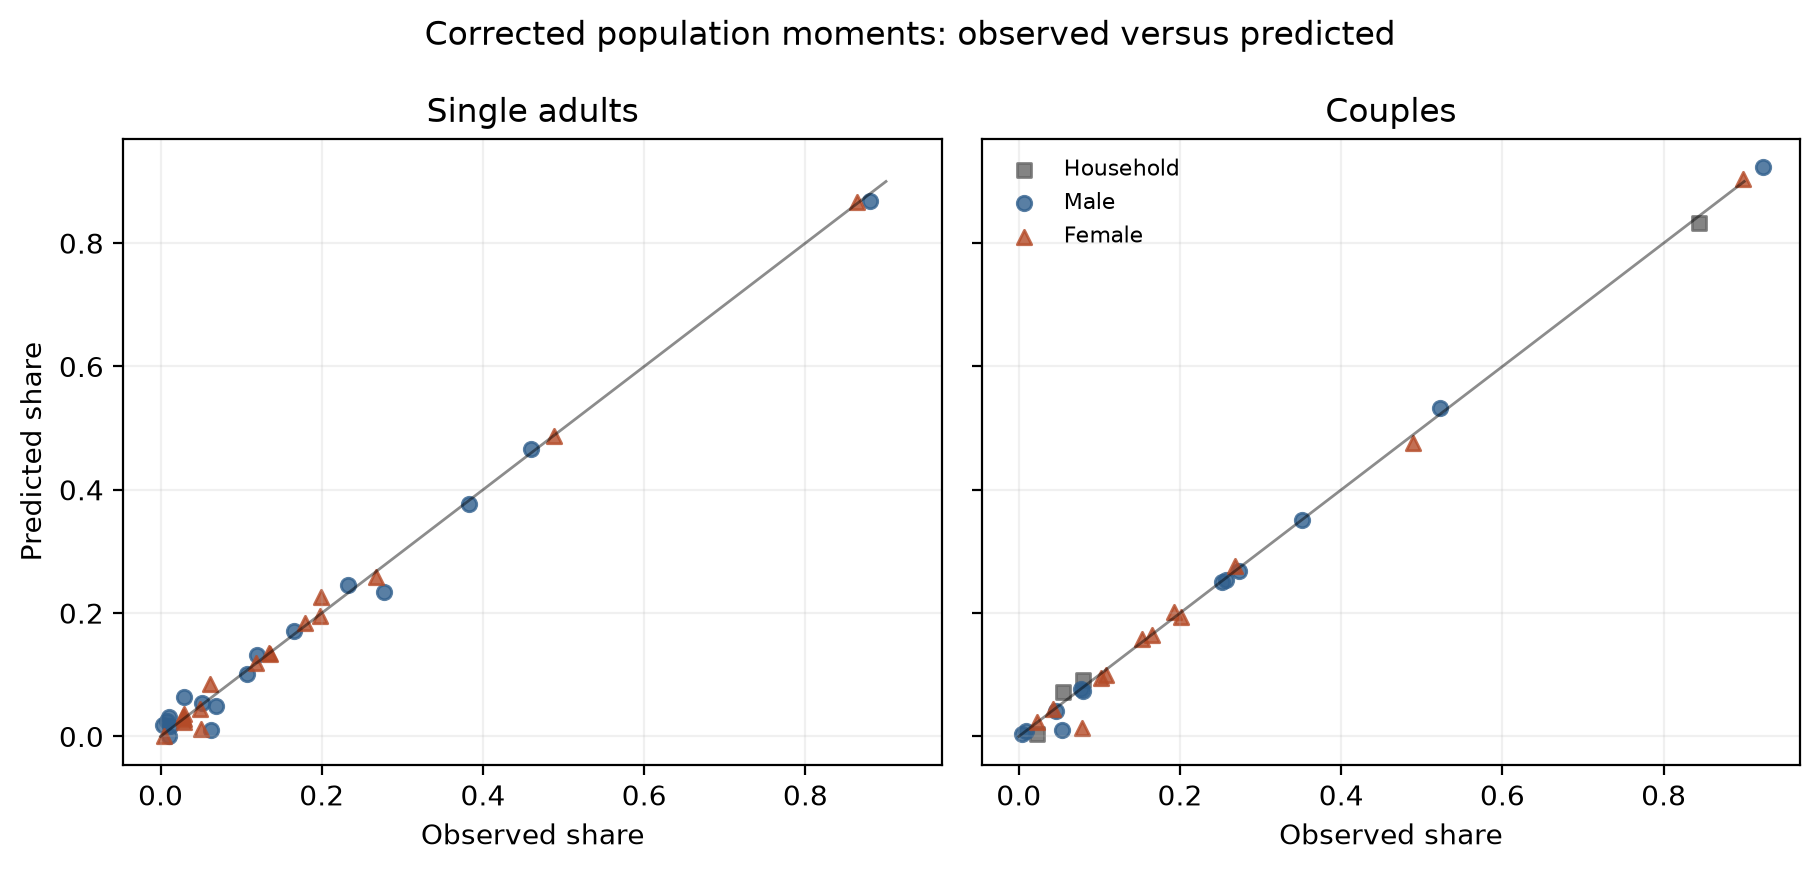
\includegraphics[height=0.72\textheight,width=\textwidth,keepaspectratio]{fit_by_margin_v7.png}
\end{center}
\backnav{main:est}
\note{Corrected population fit: observed against predicted shares, margin by
margin. Participation and occupation margins are reproduced closely in aggregate;
the hours fit is uneven. Population predictions integrate the model over
opportunities and taste shocks, so this is not an in-sample fitted choice.}
\end{frame}

\begin{frame}
\frametitle{Backup: the thirty-seven-hour point}
\hypertarget{b:hours37}{}
\vfill
\begin{columns}[T,onlytextwidth]
\column{0.23\textwidth}\centering
\textbf{single men}\\[0.3em]{\Large \VGapSingleMen} \\ {\footnotesize pp}
\column{0.23\textwidth}\centering
\textbf{single women}\\[0.3em]{\Large \VGapSingleWomen} \\ {\footnotesize pp}
\column{0.23\textwidth}\centering
\textbf{coupled men}\\[0.3em]{\Large \VGapCoupledMen} \\ {\footnotesize pp}
\column{0.23\textwidth}\centering
\textbf{coupled women}\\[0.3em]{\Large \VGapCoupledWomen} \\ {\footnotesize pp}
\end{columns}
\vfill
\begin{center}
{\small observed minus predicted share at the observed thirty-seven-hour mass point}
\end{center}
\vfill
\backnav{main:est}
\note{The common hours mismatch is underprediction of the observed concentration
at exactly thirty-seven hours. It is a finding about that mass point, not about
the model's neighbouring full-time range, and it is kept as its own result.}
\end{frame}

\begin{frame}
\frametitle{Backup: matched households}
\hypertarget{b:matched}{}
\begin{center}
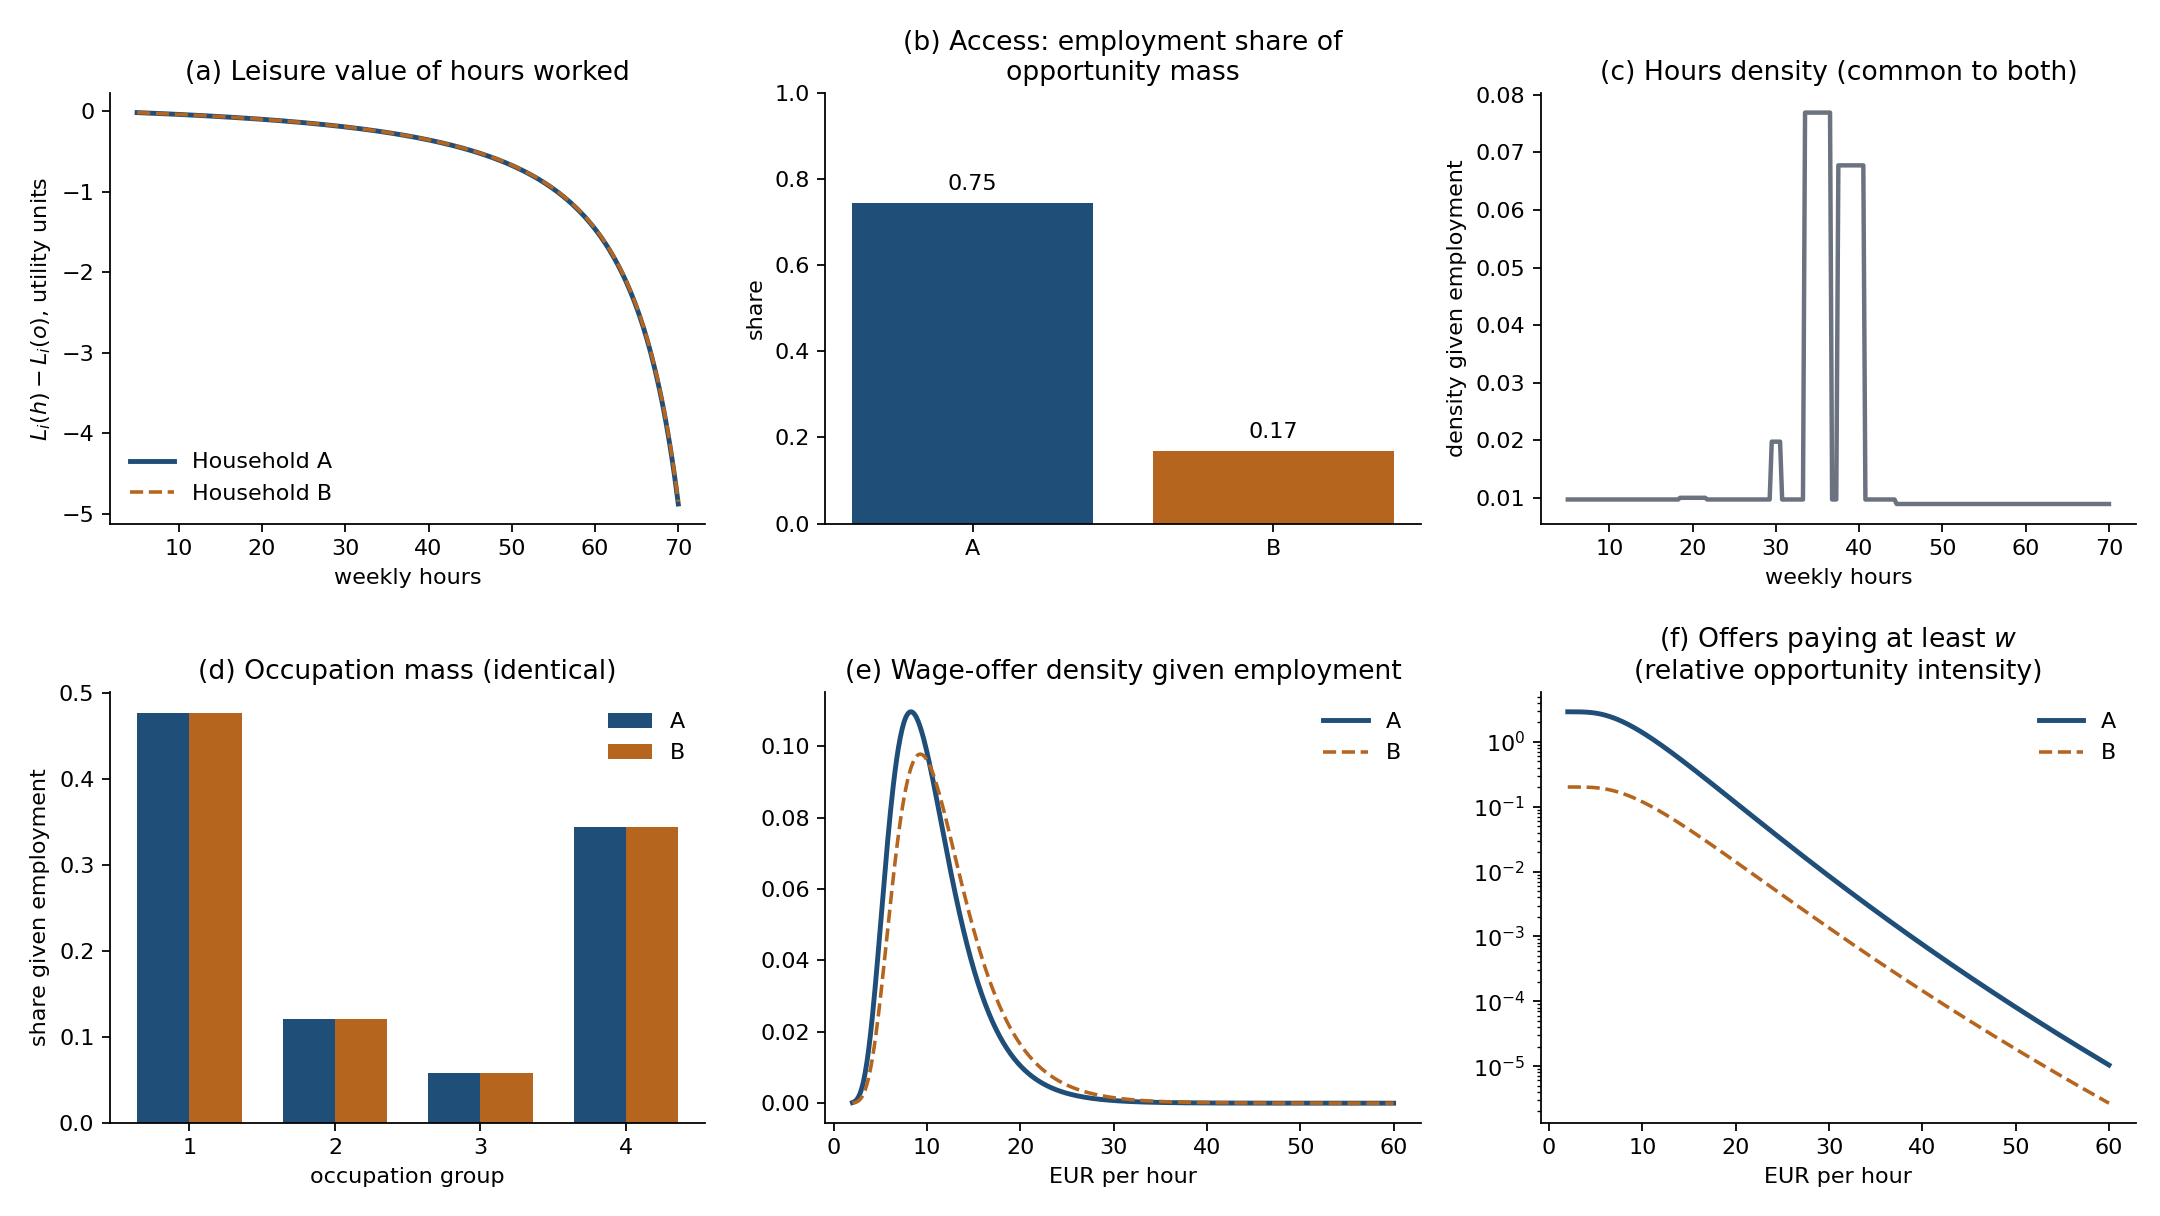
\includegraphics[height=0.64\textheight,width=\textwidth,keepaspectratio]{fig_matched_households_v11.png}
\end{center}
\begin{center}
{\footnotesize access: A $=$ \VMatchedAccessRatio{} $\times$ B \qquad wage-offer location: B $+$\VMatchedWageGap{} log points}
\end{center}
\backnav{main:opp}
\note{What unequal opportunity means inside the model. Two employed single men in
the same occupation group, hours band and wage quintile, with nearly identical
estimated leisure profiles, selected by a stated rule: a teaching example, not
causal and not representative. Employment is \VMatchedEmpShareA{} of A's
opportunity mass and \VMatchedEmpShareB{} of B's. B's wage offers are better, yet
A faces more offers paying at least any given wage over essentially all offer
mass. Neither is better placed on every margin.}
\end{frame}

\begin{frame}
\frametitle{Backup: marginal rate of substitution}
\hypertarget{b:mrs}{}
\begin{center}
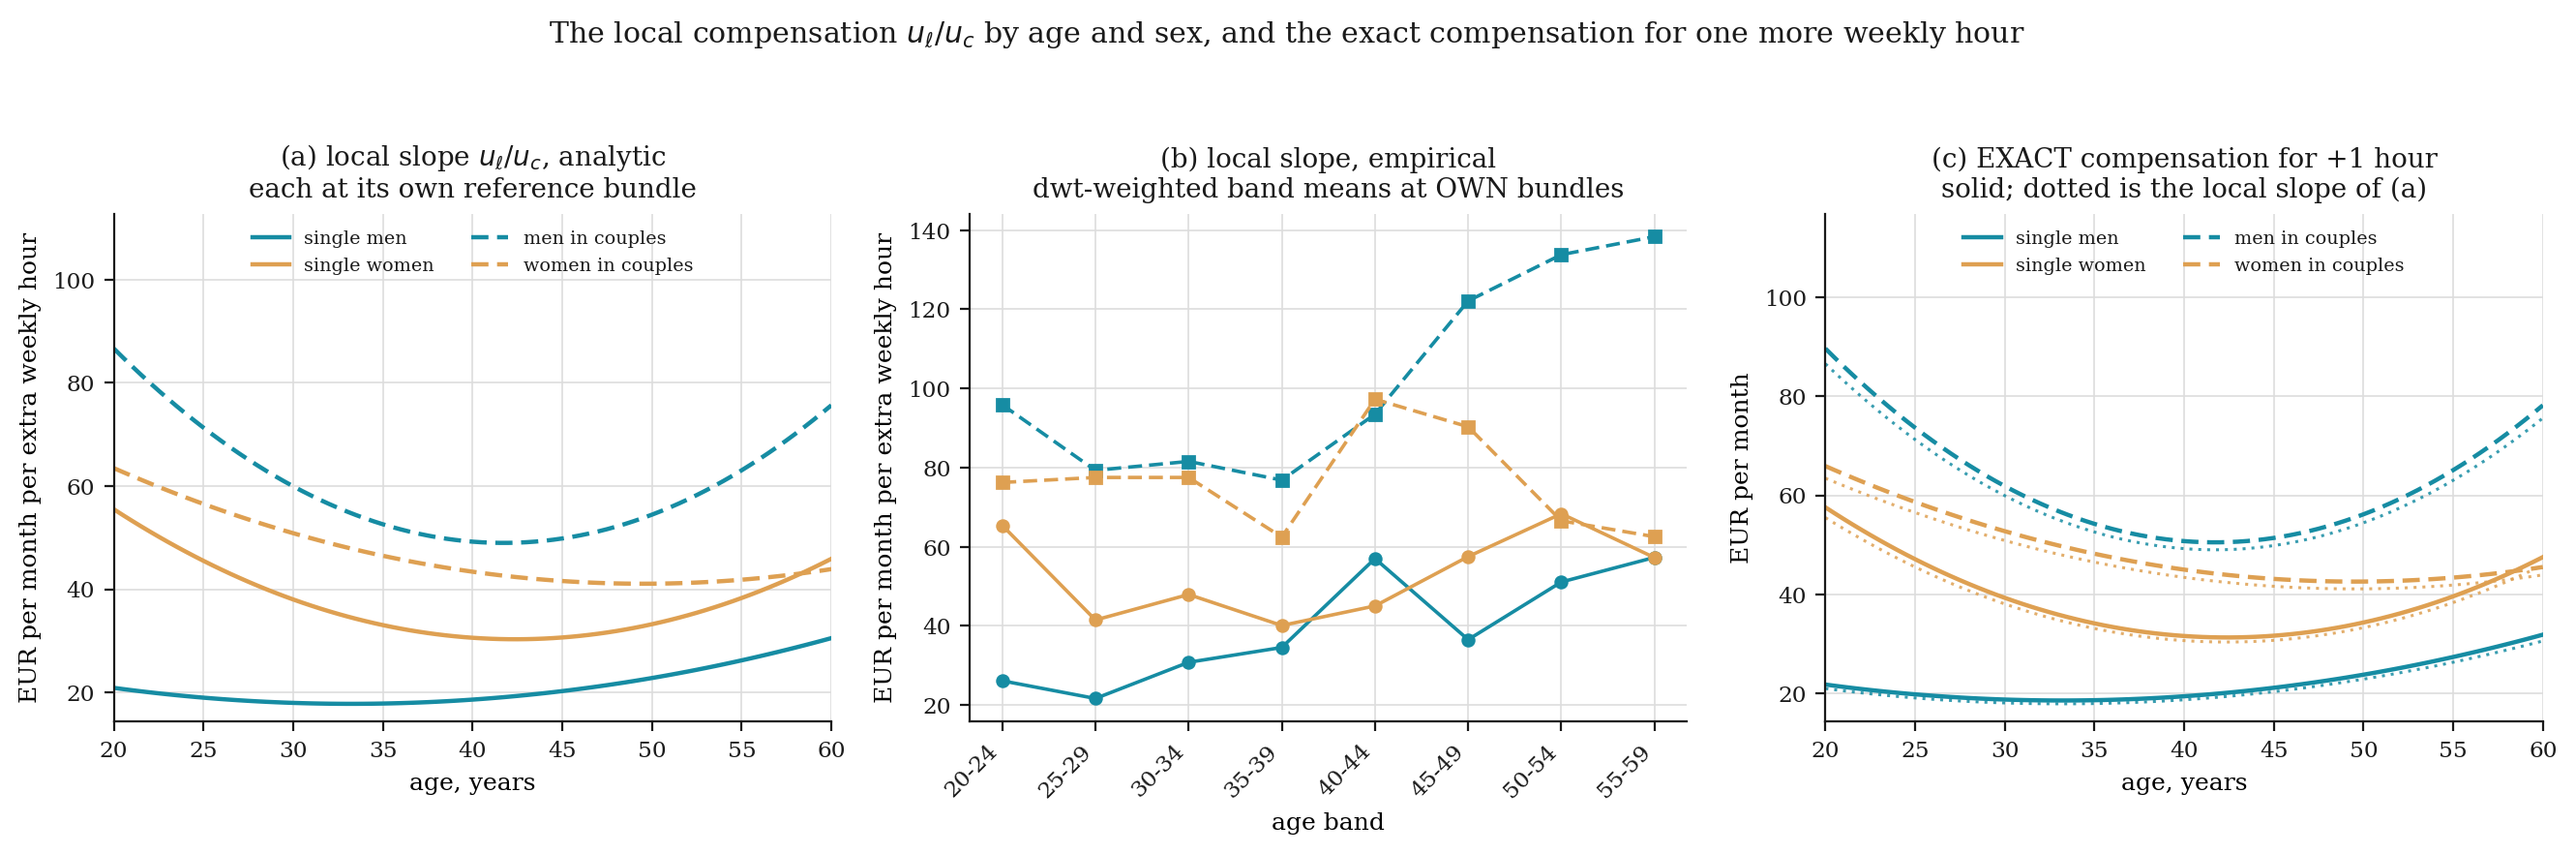
\includegraphics[height=0.72\textheight,width=\textwidth,keepaspectratio]{figP04_mrs_by_age_sex.png}
\end{center}
\backnav{main:sel}
\note{The marginal rate of substitution between leisure and consumption, by age
and sex, in euros per month per additional recurring weekly hour of leisure. It is
a compensation along an indifference curve, not a behavioural response to a wage
change. The coefficients are coordinates; this is the economics.}
\end{frame}

% ==================================================================== WELFARE
\begin{frame}
\frametitle{Backup: attained-bundle derivation}
\hypertarget{b:attderiv}{}
\vfill
\backupeq{$\displaystyle L_i(o)+\beta_c\log\!\Big(\frac{M^{\mathrm{att}}_i}{\lambda_c}\Big)=L_i(j^{\mathrm{obs}}_i)+\beta_c\log\!\Big(\frac{C^{\mathrm{obs}}_i}{\lambda_c}\Big)$}
\backupeq{$\displaystyle\Longrightarrow\quad M^{\mathrm{att}}_i=C^{\mathrm{obs}}_i\exp\!\Big\{\frac{L_i(j^{\mathrm{obs}}_i)-L_i(o)}{\beta_c}\Big\}$}
\vfill
\begin{columns}[T,onlytextwidth]
\column{0.46\textwidth}\centering
\textbf{Reference job}\\ {\footnotesize the preferred job when every job pays the same: here non-employment for every household}
\column{0.46\textwidth}\centering
\textbf{Staying-home equivalent}\\ {\footnotesize a verified property of this specification, not a general theorem}
\end{columns}
\vfill
\backnav{main:att}
\note{The attained-bundle money metric solves an indifference condition between
the observed job and consumption and the reference state at the unknown
consumption. The normaliser cancels. The general construction uses the job the
household would most prefer at equal pay; on the current domain non-employment
maximises the non-consumption index for every household, so the measure is the
staying-home equivalent. With a different leisure specification the two could
separate.}
\end{frame}

\begin{frame}
\frametitle{Backup: ex-ante derivation}
\hypertarget{b:eaderiv}{}
\vfill
\backupeq{$\displaystyle J_i=\int_{\Omega_i}e^{L_i(j)}\Big(\frac{C_i(j)}{\lambda_c}\Big)^{\beta_c}\widehat g_i(j)\,d\nu(j)$}
\backupeq{$\displaystyle J^{\mathrm{ref}}_i(m)=\Big(\frac{m}{\lambda_c}\Big)^{\beta_c}H_i,\qquad H_i=\int_{\Omega_i}e^{L_i(j)}\,\widehat g_i(j)\,d\nu(j)$}
\backupeq{$\displaystyle J^{\mathrm{ref}}_i\big(M^{\mathrm{EA}}_i\big)=J_i\quad\Longrightarrow\quad M^{\mathrm{EA}}_i=\lambda_c\exp\!\Big\{\frac{\log J_i-\log H_i}{\beta_c}\Big\}$}
\vfill
\begin{center}
{\small a common rescaling of $\widehat g_i$ cancels \quad$\cdot$\quad $\log J_i$: expected utility of the best reachable job, up to a constant}
\end{center}
\vfill
\backnav{main:ea}
\note{The reference prospect keeps the household's jobs, availability and
preferences and pays the same consumption at every job; its value is the power
of that consumption times H. Setting it equal to the actual prospect and solving
gives the ex-ante money metric. Under the extreme-value shocks, log J is the
expected utility of the best reachable job up to a constant common to J and H,
which is why taste-shock variety counts as welfare-relevant: a normative
position.}
\end{frame}

\begin{frame}
\frametitle{Backup: ex-ante numerical validation}
\hypertarget{b:eavalid}{}
\vfill
\begin{columns}[T,onlytextwidth]
\column{0.46\textwidth}
\centering
\textbf{Identities}\\[0.5em]
{\small constant-consumption identity}\\
{\small one-state identity}\\
{\small common intensity-rescaling invariance}\\
{\small flat-reference inversion}\\
{\small exact Shapley adding-up}
\column{0.46\textwidth}
\centering
\textbf{Numerics}\\[0.5em]
{\small exact reference integral on the priced set}\\
{\small effective sample size and weight concentration}\\
{\small two-seed stability of welfare, Gini and Shapley}\\
{\small finite positive welfare for every household}\\
{\small independent reimplementation}
\end{columns}
\vfill
\begin{center}
{\small all passed for both populations \quad$\cdot$\quad a correct computation, not causal identification or parameter uncertainty}
\end{center}
\vfill
\backnav{main:ea}
\note{The ex-ante calculation passed every declared check for both populations,
including an independent reimplementation, with the integration design fixed
before inspecting any welfare level or Shapley value. That certifies the
computation given the model and operators. It does not establish causal
identification, it does not quantify statistical uncertainty in the estimated
parameters, and it does not make either welfare perspective normatively correct.
Channel orderings are unchanged across the reported reference-domain
sensitivities.}
\end{frame}

\begin{frame}
\frametitle{Backup: equivalisation}
\hypertarget{b:equiv}{}
\vfill
\backupeq{$\displaystyle M^{p,\mathrm{eq}}_i=\frac{M^p_i}{e_i},\qquad e_i:\ \text{modified-OECD scale}$}
\vfill
\begin{columns}[T,onlytextwidth]
\column{0.46\textwidth}
\centering
\textbf{Couples, ex ante: A + B}\\[0.5em]
{\large \VEACoupOppRaw{}\% \quad$\longrightarrow$\quad \VEACoupOppEq{}\%}\\[0.3em]
{\footnotesize raw \quad$\to$\quad equivalised; \% of baseline Gini}
\column{0.46\textwidth}
\centering
\textbf{Couples, ex ante: preferences}\\[0.5em]
{\large \VEACoupPrefRaw{} \quad$\longrightarrow$\quad \VEACoupPrefEq{}}\\[0.3em]
{\footnotesize Gini points, raw \quad$\to$\quad equivalised}
\end{columns}
\vfill
\begin{center}
{\small a normative convention, reported both ways; populations never combined or compared}
\end{center}
\vfill
\backnav{main:howmuch}
\note{Equivalisation is a normative convention and it is consequential for couples
under the ex-ante perspective: it moves access plus earnings as a share of
baseline inequality and turns the preference contribution negative. A negative
Shapley term means that, averaged over orders, equalising preferences raises
inequality; it does not show that preference heterogeneity is equalising in any
causal or welfare sense. That is why both scales are always reported.}
\end{frame}

% ==================================================================== DECOMPOSITION
\begin{frame}
\frametitle{Backup: central figure}
\hypertarget{b:central}{}
\begin{center}
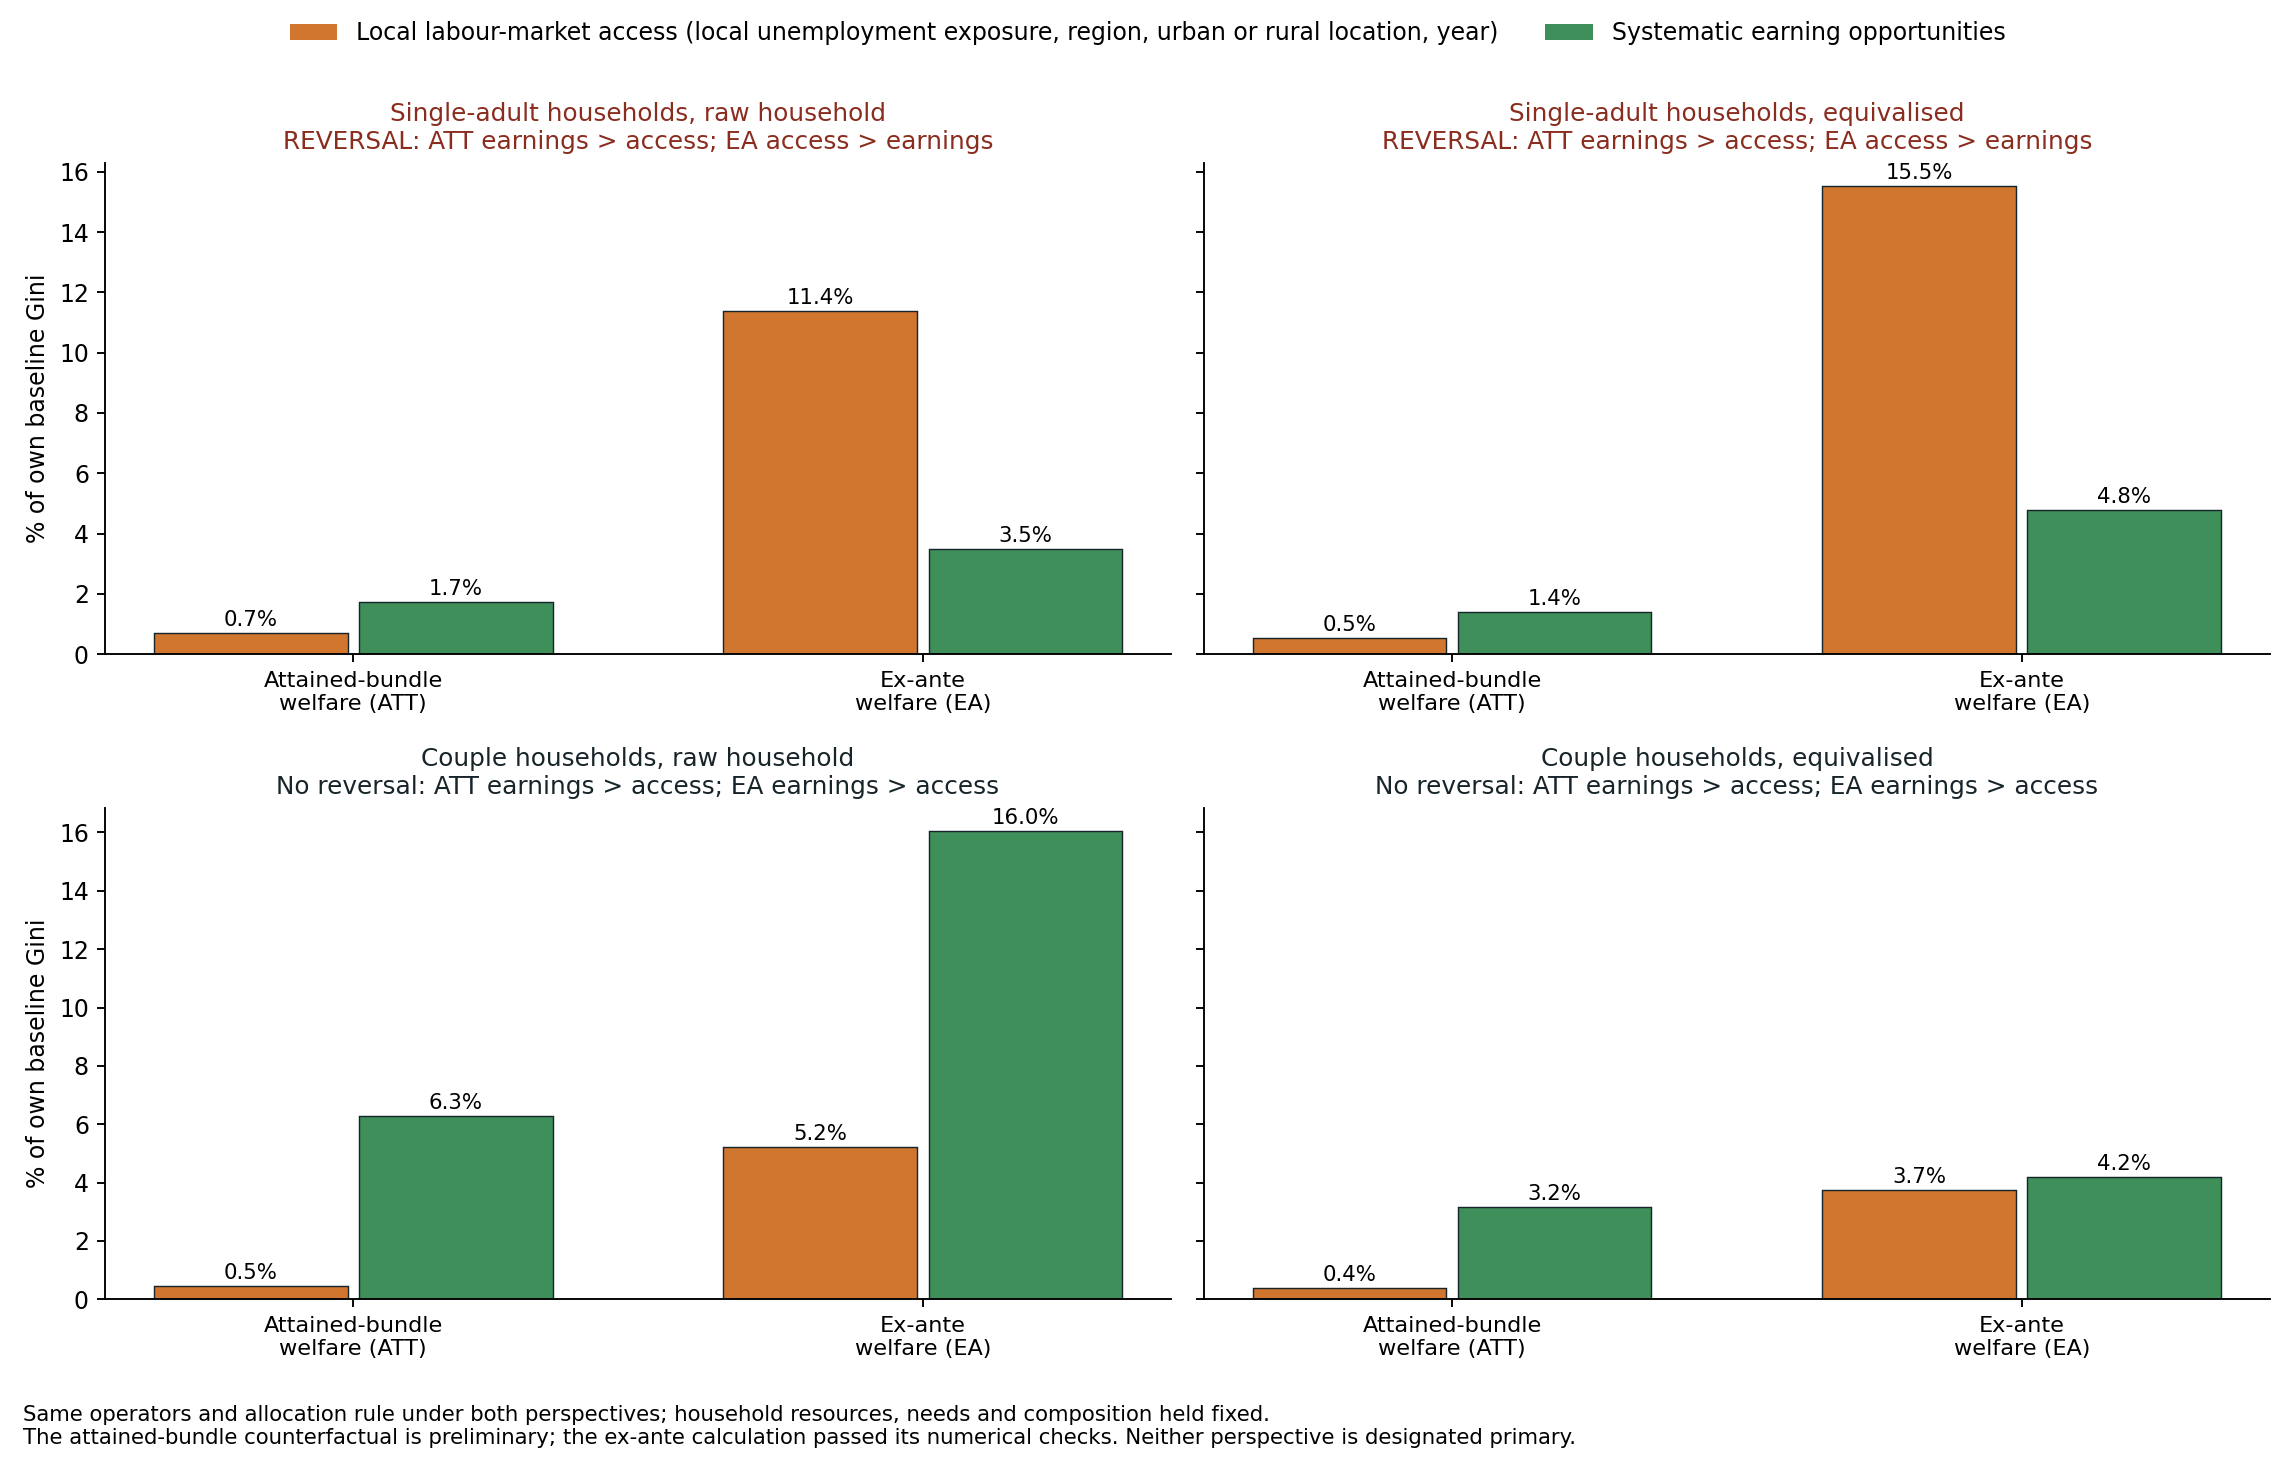
\includegraphics[height=0.72\textheight,width=\textwidth,keepaspectratio]{fig_v13_central_result.png}
\end{center}
\backnav{main:howmuch}
\note{The published central figure: access and earning-opportunity contributions,
each as a percentage of its own perspective's baseline Gini, under attained-bundle
and ex-ante welfare, raw and equivalised. For single adults earning
opportunities are larger under the attained bundle and access is larger under
the prospect; couples show no reversal. Resources, needs and composition are
held fixed.}
\end{frame}

\begin{frame}
\frametitle{Backup: ex-ante decomposition in Gini points}
\hypertarget{b:eagini}{}
\vfill
\begin{center}\scriptsize
\renewcommand{\arraystretch}{1.25}
\setlength{\tabcolsep}{4pt}
\begin{tabular}{llcccccl}
\toprule
 & scale & baseline Gini & \textcolor{chpref}{P} & \textcolor{chacc}{A} & \textcolor{chearn}{B} & A + B, \% of baseline & ordering \\
\midrule
Single adults & raw & \VEASingGiniRaw & \VEASingPhiPRaw & \VEASingPhiARaw & \VEASingPhiBRaw & \VEASingOppRaw & access $>$ earnings \\
 & equivalised & \VEASingGiniEq & \VEASingPhiPEq & \VEASingPhiAEq & \VEASingPhiBEq & \VEASingOppEq & access $>$ earnings \\
\midrule
Couples & raw & \VEACoupGiniRaw & \VEACoupPhiPRaw & \VEACoupPhiARaw & \VEACoupPhiBRaw & \VEACoupOppRaw & earnings $>$ access \\
 & equivalised & \VEACoupGiniEq & \VEACoupPhiPEq & \VEACoupPhiAEq & \VEACoupPhiBEq & \VEACoupOppEq & earnings $>$ access \\
\bottomrule
\end{tabular}
\end{center}
\vfill
{\footnotesize exact Shapley contributions in Gini points; household-weighted}
\backnav{main:howmuch}
\note{The full ex-ante table. Contributions are signed Gini points; access plus
earnings is reported relative to each baseline Gini. The calculation passed its
numerical checks, including an independent implementation. For couples the
preference contribution changes sign with equivalisation.}
\end{frame}

\begin{frame}
\frametitle{Backup: attained-bundle decomposition in Gini points}
\hypertarget{b:attgini}{}
\vfill
\begin{center}\scriptsize
\renewcommand{\arraystretch}{1.25}
\setlength{\tabcolsep}{4pt}
\begin{tabular}{llcccccl}
\toprule
 & scale & baseline Gini & \textcolor{chpref}{P} & \textcolor{chacc}{A} & \textcolor{chearn}{B} & A + B, \% of baseline & ordering \\
\midrule
Single adults & raw & \VAttFigSingGiniRaw & \VAttFigSingPhiPRaw & \VAttFigSingPhiARaw & \VAttFigSingPhiBRaw & \VAttSingOppRaw & earnings $>$ access \\
 & equivalised & \VAttFigSingGiniEq & \VAttFigSingPhiPEq & \VAttFigSingPhiAEq & \VAttFigSingPhiBEq & \VAttSingOppEq & earnings $>$ access \\
\midrule
Couples & raw & \VAttFigCoupGiniRaw & \VAttFigCoupPhiPRaw & \VAttFigCoupPhiARaw & \VAttFigCoupPhiBRaw & \VAttCoupOppRaw & earnings $>$ access \\
 & equivalised & \VAttFigCoupGiniEq & \VAttFigCoupPhiPEq & \VAttFigCoupPhiAEq & \VAttFigCoupPhiBEq & \VAttCoupOppEq & earnings $>$ access \\
\bottomrule
\end{tabular}
\end{center}
\vfill
{\footnotesize exact Shapley contributions in Gini points; preliminary; household-weighted}
\backnav{main:howmuch}
\note{The attained-bundle table. Earning opportunities are larger than local
access for both household types and both scales. The preference contribution
changes sign with equivalisation in both samples, so no directional claim is made
about it. The lower part of the hours range is sparsely represented in the
integration sample, which is why this exercise stays preliminary.}
\end{frame}

\begin{frame}
\frametitle{Backup: ex-ante channels, \% of baseline}
\hypertarget{b:eapct}{}
\vfill
\begin{center}\footnotesize
\renewcommand{\arraystretch}{1.3}
\setlength{\tabcolsep}{4pt}
\begin{tabular}{llc cc cc cc}
\toprule
 & & & \multicolumn{2}{c}{\textcolor{chpref}{P}} & \multicolumn{2}{c}{\textcolor{chacc}{A}} & \multicolumn{2}{c}{\textcolor{chearn}{B}} \\
 & scale & $I_0$ & Gini pts & \% of $I_0$ & Gini pts & \% of $I_0$ & Gini pts & \% of $I_0$ \\
\midrule
Single adults & raw & \VEASingGiniRaw & \VEASingPhiPRaw & \VPctEASingPRaw & \VEASingPhiARaw & \VPctEASingARaw & \VEASingPhiBRaw & \VPctEASingBRaw \\
 & equivalised & \VEASingGiniEq & \VEASingPhiPEq & \VPctEASingPEq & \VEASingPhiAEq & \VPctEASingAEq & \VEASingPhiBEq & \VPctEASingBEq \\
\midrule
Couples & raw & \VEACoupGiniRaw & \VEACoupPhiPRaw & \VPctEACoupPRaw & \VEACoupPhiARaw & \VPctEACoupARaw & \VEACoupPhiBRaw & \VPctEACoupBRaw \\
 & equivalised & \VEACoupGiniEq & \VEACoupPhiPEq & \VPctEACoupPEq & \VEACoupPhiAEq & \VPctEACoupAEq & \VEACoupPhiBEq & \VPctEACoupBEq \\
\bottomrule
\end{tabular}
\end{center}
\vfill
{\footnotesize each contribution divided by its own baseline Gini $I_0$; signed; the rows are not forced to sum to one hundred, because the remainder is outside the current P-A-B decomposition}
\cornerlinks{\hyperlink{main:channel}{\beamerreturnbutton{Back}}\ \hyperlink{appmap}{\beamergotobutton{Appendix map}}\ \golink{b:explained}{composition within P/A/B}}
\note{Each ex-ante Shapley contribution, in Gini points and as a percentage of its
own baseline Gini, raw and equivalised. The negative couples preference term is
kept. P, A and B do not exhaust baseline inequality: household resources, needs
and composition and other dimensions are held fixed or left unallocated.}
\end{frame}

\begin{frame}
\frametitle{Backup: attained-bundle channels, \% of baseline}
\hypertarget{b:attpct}{}
\vfill
\begin{center}\footnotesize
\renewcommand{\arraystretch}{1.3}
\setlength{\tabcolsep}{4pt}
\begin{tabular}{llc cc cc cc}
\toprule
 & & & \multicolumn{2}{c}{\textcolor{chpref}{P}} & \multicolumn{2}{c}{\textcolor{chacc}{A}} & \multicolumn{2}{c}{\textcolor{chearn}{B}} \\
 & scale & $I_0$ & Gini pts & \% of $I_0$ & Gini pts & \% of $I_0$ & Gini pts & \% of $I_0$ \\
\midrule
Single adults & raw & \VAttFigSingGiniRaw & \VAttFigSingPhiPRaw & \VPctAttSingPRaw & \VAttFigSingPhiARaw & \VPctAttSingARaw & \VAttFigSingPhiBRaw & \VPctAttSingBRaw \\
 & equivalised & \VAttFigSingGiniEq & \VAttFigSingPhiPEq & \VPctAttSingPEq & \VAttFigSingPhiAEq & \VPctAttSingAEq & \VAttFigSingPhiBEq & \VPctAttSingBEq \\
\midrule
Couples & raw & \VAttFigCoupGiniRaw & \VAttFigCoupPhiPRaw & \VPctAttCoupPRaw & \VAttFigCoupPhiARaw & \VPctAttCoupARaw & \VAttFigCoupPhiBRaw & \VPctAttCoupBRaw \\
 & equivalised & \VAttFigCoupGiniEq & \VAttFigCoupPhiPEq & \VPctAttCoupPEq & \VAttFigCoupPhiAEq & \VPctAttCoupAEq & \VAttFigCoupPhiBEq & \VPctAttCoupBEq \\
\bottomrule
\end{tabular}
\end{center}
\vfill
{\footnotesize each contribution divided by its own baseline Gini $I_0$; signed; preliminary}
\backnav{main:channel}
\note{The same layout for the attained-bundle perspective. Earning opportunities
exceed access in every row; the preference contribution changes sign with
equivalisation. These percentages are shares of each baseline Gini and are not
forced to sum to one hundred.}
\end{frame}

\begin{frame}
\frametitle{Backup: composition of the explained component}
\hypertarget{b:explained}{}
\vfill
\backupeq{$\displaystyle s_k=\frac{\phi_k}{\phi_P+\phi_A+\phi_B},\qquad k\in\{P,A,B\}$}
\vfill
\begin{center}\small
\renewcommand{\arraystretch}{1.35}
\begin{tabular}{lrr}
\toprule
ex-ante prospect, equivalised & Single adults & Couples \\
\midrule
\textcolor{chpref}{Preferences} $s_P$ & \VExplSingP\% & \VExplCoupP\% \\
\textcolor{chacc}{Local access} $s_A$ & \VExplSingA\% & \VExplCoupA\% \\
\textcolor{chearn}{Earning opportunities} $s_B$ & \VExplSingB\% & \VExplCoupB\% \\
\midrule
Total & \VExplSingTotal\% & \VExplCoupTotal\% \\
\bottomrule
\end{tabular}
\end{center}
\vfill
{\footnotesize These are shares of the currently explained P/A/B change, not shares of total inequality. Negative components are possible under Shapley attribution.\par}
\backnav{b:eapct}
\note{These are shares of the currently explained P/A/B change, not shares of
total inequality. Negative components are possible under Shapley attribution.

Within that currently explained component, most of the single-adult opportunity
effect comes through access rather than earning opportunities. For couples the
negative preference share means the access and earning shares together exceed
the whole explained change. Only the equivalised scale is shown: on the raw scale
the one-decimal couples shares would not close exactly.}
\end{frame}

\begin{frame}
\frametitle{Backup: Shapley versus one-factor equalisation}
\hypertarget{b:shapley}{}
\vfill
\backupeq{$\displaystyle \text{one-factor:}\quad v^p(\{k\})=I^p(\varnothing)-I^p(\{k\})$}
\backupeq{$\displaystyle \text{Shapley:}\quad \phi^p_k=\text{average over all orders of } v^p(S\cup\{k\})-v^p(S)$}
\backupeq{$\displaystyle \phi^p_P+\phi^p_A+\phi^p_B=I^p(\varnothing)-I^p(\{P,A,B\})$}
\vfill
\begin{center}
{\small one-factor effects need not add up \quad$\cdot$\quad Shapley contributions do, exactly}
\end{center}
\vfill
\backnav{main:shapley}
\note{A one-factor effect equalises one channel from the actual situation. Because
the channels interact, those effects need not add up, and the answer would depend
on the order chosen. The Shapley contribution averages each channel's marginal
effect over every order and adds up exactly to the total change. This is the
standard rule from the distributional decomposition literature; no new principle
is claimed. Coalition-by-coalition Gini tables are not reproduced in these
slides.}
\end{frame}

\begin{frame}
\frametitle{Backup: outside the current P-A-B decomposition}
\hypertarget{b:residual}{}
\vfill
\begin{columns}[T,onlytextwidth]
\column{0.31\textwidth}\centering
\textbf{Held fixed}\\[0.4em]
{\footnotesize household resources, needs and composition}
\column{0.31\textwidth}\centering
\textbf{Retained}\\[0.4em]
{\footnotesize sex-specific and household-type-specific preference and opportunity blocks}
\column{0.31\textwidth}\centering
\textbf{Not equalised}\\[0.4em]
{\footnotesize wage-draw luck and the common offer spread}
\end{columns}
\vfill
\begin{center}
wage-offer location differences: at most about \VOfferLocation{} log points\\[0.3em]
common offer spread: about \VOfferSpread{} log points
\end{center}
\vfill
\begin{center}
{\small next: extend the decomposition to household resources and needs, after fixing the appropriate operator}
\end{center}
\backnav{main:hundred}
\note{The last row of the percentage display is everything the current
decomposition does not equalise. It is not a channel. It holds household
resources, needs and composition fixed, it keeps the sex-specific and
household-type-specific blocks, and it excludes wage-draw luck and the common
offer spread. The location differences that the earning operator equalises are
small next to that common spread, so the operator removes only a small part of
earnings dispersion by construction. Extending the decomposition to household
resources and needs requires fixing the appropriate operator first, because some
covariates enter both preferences and needs; until then there is no fourth
channel to allocate.}
\end{frame}

\begin{frame}
\frametitle{Backup: robustness of the attained-bundle decomposition}
\hypertarget{b:robust}{}
\vfill
\begin{columns}[T,onlytextwidth]
\column{0.46\textwidth}
\centering
\textbf{Second simulation seed}\\[0.5em]
{\small every coalition Gini and contribution reproduces closely, including the preference sign change}
\column{0.46\textwidth}
\centering
\textbf{Observed job in the simulation}\\[0.5em]
{\small attained under every coalition by \VObsJobShareSingles\% of single adults and \VObsJobShareCouples\% of couples}\\[0.3em]
{\small excluding it moves the total change by at most \VObsJobMove\%, with no sign change}
\end{columns}
\vfill
\begin{center}
{\small simulation checks, not confidence intervals}
\end{center}
\vfill
\backnav{main:limits}
\note{Robustness of the attained-bundle calculation. An independent second seed
reproduces every coalition Gini and Shapley contribution closely. The simulation
always includes each household's own observed job; excluding it moves the total
change by at most the amount shown, in the couples equivalised case, with no sign
change. These checks validate the calculation for the stated game, not its
maintained assumptions, and they are not confidence intervals.}
\end{frame}

% ==================================================================== DATA
\begin{frame}
\frametitle{Backup: sample selection}
\hypertarget{b:sample}{}
\vfill
\begin{center}\scriptsize
\renewcommand{\arraystretch}{1.15}
\begin{tabular}{>{\raggedright\arraybackslash}p{0.56\textwidth}rr}
\toprule
screen & single-adult & couple \\
\midrule
\VFunnelZeroLabel & \VFunnelZeroSingles & \VFunnelZeroCouples \\
\VFunnelOneLabel & \VFunnelOneSingles & \VFunnelOneCouples \\
\VFunnelTwoLabel & \VFunnelTwoSingles & \VFunnelTwoCouples \\
\VFunnelThreeLabel & \VFunnelThreeSingles & \VFunnelThreeCouples \\
\VFunnelFourLabel & \VFunnelFourSingles & \VFunnelFourCouples \\
\VFunnelFiveLabel & \VFunnelFiveSingles & \VFunnelFiveCouples \\
\VFunnelSixLabel & \VFunnelSixSingles & \VFunnelSixCouples \\
\VFunnelSevenLabel & \VFunnelSevenSingles & \VFunnelSevenCouples \\
\VFunnelEightLabel & \VFunnelEightSingles & \VFunnelEightCouples \\
\VFunnelNineLabel & \VFunnelNineSingles & \VFunnelNineCouples \\
\midrule
\textbf{estimation sample} & \textbf{\VNSingles} & \textbf{\VNCouples} \\
\bottomrule
\end{tabular}
\end{center}
\vfill
\backnav{main:data}
\note{Unweighted households remaining after each screen. The largest exclusion is
structural: multi-generational households, flat-shares and same-sex couples are
outside the estimated population, and no result extends to them. Students and
pension recipients are removed because the model does not define an offer set for
them; the remaining screens are support restrictions.}
\end{frame}

\begin{frame}
\frametitle{Backup: EUROMOD pricing}
\hypertarget{b:pricing}{}
\vfill
\begin{columns}[T,onlytextwidth]
\column{0.31\textwidth}\centering
\textbf{Inputs}\\[0.4em]
{\footnotesize a work arrangement: hours, hourly wage, earnings split; household roster and non-labour inputs}
\column{0.31\textwidth}\centering
\textbf{EUROMOD}\\[0.4em]
{\footnotesize French \VPolicyYear{} policy system; only deciders receive counterfactual overrides}
\column{0.31\textwidth}\centering
\textbf{Output}\\[0.4em]
{\footnotesize $C_i(j)$: household disposable income, summed over all members}
\end{columns}
\vfill
\begin{center}
{\small every sampled alternative and every welfare integration point is priced}\\[0.3em]
{\small tax-benefit accounting identity holds to machine precision}
\end{center}
\vfill
\backnav{main:data}
\note{For a given work arrangement the tax-benefit model receives the implied
gross labour inputs together with the household's non-labour inputs and roster,
and returns disposable income. Only deciders receive counterfactual overrides;
other members keep their baseline values. The accounting identity linking
original income, benefits, taxes and contributions to disposable income holds to
machine precision at the person and household-alternative level.}
\end{frame}

\begin{frame}
\frametitle{Backup: numerical design}
\hypertarget{b:numerics}{}
\vfill
\begin{columns}[T,onlytextwidth]
\column{0.31\textwidth}\centering
\textbf{Estimation}\\[0.4em]
{\Large \VNAltRows}\\ {\footnotesize rows per household: the observed job and \VNDraws{} sampled alternatives}
\column{0.31\textwidth}\centering
\textbf{Predictive fit}\\[0.4em]
{\Large \VNNodes}\\ {\footnotesize common integration points per household}
\column{0.31\textwidth}\centering
\textbf{Supports}\\[0.4em]
{\Large $[\VHoursFloor,\VHoursCap]$}\\ {\footnotesize weekly hours; wages in $[\VWageLo,\VWageHi]$ per hour}
\end{columns}
\vfill
\begin{center}
{\small sampling devices are computational: they are not offers and enter no welfare measure}
\end{center}
\vfill
\backnav{main:data}
\note{The numerical design. Estimation uses the observed job plus sampled
alternatives per household. The predictive fit integrates over a separate, larger
common set of priced integration points per household. The supports are the
intervals on which the opportunity densities are defined. The ex-ante welfare
integrals use their own certified design, chosen before any welfare result was
inspected.}
\end{frame}

\end{document}
